\section*{Chapter declaration}
\addcontentsline{toc}{section}{\numberline{}Chapter declaration}
The data, analysis, results, and discussion presented in this chapter were reported in my first-author publication ``Outflow densities and ionization mechanisms in the NLRs of the prototypical Seyfert galaxies NGC 1068 and NGC 4151'' \citep{HoldenTadhunter2023}. The content of this chapter is based on that publication, which has been adapted into a suitable format for this thesis; all work is my own, except where clearly stated.

\newpage

\section[Chapter introduction]{Chapter introduction: the prototypical Seyfert galaxies NGC\;1068 \& NGC\;4151}
\label{section: stis_seyferts: introduction}

In Chapter \ref{chapter: xshooter_ic5063}, I presented a detailed study of the jet-driven outflows in the NLR of the nearby Sey\;2 galaxy IC\;5063 using \mbox{Very Large Telescope (VLT) / Xshooter} ultraviolet (UV), optical and near-infrared (NIR) spectroscopy. Electron densities above the sensitivity limit of the traditional [SII] ratio were found --- resulting in modest warm-ionised outflow kinetic powers ($\dot{E}_\mathrm{kin}=(2.7\pm1.7)\times10^{-3}$ of $L_\mathrm{bol}$) --- in addition to AGN-photoionisation being the dominant ionisation mechanism.

There is now a clear need to determine whether the conditions found in the NLR of IC\;5063 are similar in other Seyfert galaxies, specifically to further investigate true outflow electron densities, kinetic powers, and ionisation mechanisms. Furthermore, considering that IC\;5063 has well-known jet-driven outflows, it is important to investigate the gas conditions and NLR properties of objects for which the outflow acceleration mechanisms are not clear, as this may further clarify the link between outflow ionisation and acceleration. Therefore, archival Hubble Space Telescope (HST) / Space Telescope Imaging Spectrograph (STIS) spectra of the inner NLRs ($r$\;\textless\;160\;kpc) of the prototypical Seyfert galaxies NGC\;1068 and NGC\;4151 are analysed in this chapter, which applies and expands upon many of the techniques presented previously.

NGC\;1068 and NGC\;4151 appeared in Carl Seyfert's original paper that established the Seyfert class (\citealt{Seyfert1943}; see Figure \ref{fig: introduction: historical_context: seyfert1943_spectra}), and are the prototypical Seyfert\;2 and Seyfert\;1 galaxies, respectively. In consequence, they are perhaps the most well-studied AGN of their types. Their close proximity to Earth and the previous, extensive multi-wavelength studies of their properties make them ideal objects for addressing the outstanding questions outlined in Section\;\ref{section: introduction: outstanding problems}: the outflows in their central regions can be spatially resolved, and measurements made with techniques such as the transauroral-line method can be compared to those obtained using other methods. Principally, this permits an assessment of the validity of different density diagnostics, as well as an investigation into the ionisation conditions (and mechanisms) of the gas.

The distances to NGC\;1068 and NGC\;4151 are taken to be $D = 13.0$\;Mpc \citep{Revalski2021} and $D = 15.8$\;Mpc \citep{Yuan2020}, respectively, which correspond to spatial scales of 0.067\;kpc/arcseconds for NGC\;1068 and 0.078\;kpc/arcseconds for NGC\;4151.

\newpage

\subsection{NGC 1068}
\label{section: stis_seyferts: ngc1068}

NGC\;1068 is one of the closest and brightest (in terms of observed flux) Seyfert 2 galaxies, allowing detailed spatially-resolved observations, and thus making it the target for extensive studies that cover a range of spatial scales at optical (e.g. \citealt{Cecil1990, Evans1991, Axon1998, Crenshaw2000a, Kraemer2000III, Das2006}), NIR (e.g. \citealt{Raban2009, MUllerSanchez2009, May2017}) and radio (e.g. \citealt{Wilson1983, Gallimore1996, GarciaBurillo2014, GarciaBurillo2019}) wavelengths. NGC\;1068 has a radio luminosity of $L_\mathrm{1.4\;GHz}=2.3\times10^{23}$\;W\;Hz$^{-1}$ \citep{Ulvestad1984}, placing it in the upper end of the radio luminosity range for Seyfert galaxies, and its high bolometric luminosity (\mbox{0.4\;\textless\;$L_\mathrm{bol}$\textless\;4.7$\times10^{45}$\;erg\;s$^{-1}$}: \citealt{Woo2002, AlonsoHerrero2011, LopezRodriguez2018, Gravity2020}) is close to the lower boundary of the luminosity range for quasars (L$_\mathrm{bol}$\;\textgreater\;10$^{45}$\;erg\;s$^{-1}$). The galaxy also has an important historical role, as it was the first object used to verify the orientation-based unified scheme for AGN (Figure\;\ref{fig: introduction: historical_context: nlr_studies: unified_scheme}: \citealt{Antonucci1985}).

The NLR of NGC\;1068 presents as an `hourglass'-shaped bicone \citep{Riffel2014, Barbosa2014, May2017} with an opening angle of $\theta \sim 40^\circ$ along PA$=30\pm2^\circ$ at an inclination of $i=5^\circ$, placing the bicone axis close to the plane of the sky and inclined $\sim$45$^\circ$ out of the galaxy's disk (\citealt{Das2006}; but see also \citealt{Crenshaw2000a}). Outflows of warm-ionised gas with velocities up to $\sim$1500\;km\;s$^{-1}$ have been detected in the bicone \citep{Crenshaw2000_N1068, Das2006}. In the NE cone, the radio axis is closely aligned with the bicone axis --- interpreted as a radio jet propagating within the hollowed-out cone --- with a radio lobe that extends just beyond the maximum extent of the cone in optical emission (\citealt{WilsonUlvestad1987}; shown in Figure\;\ref{fig: observations_and_data_reduction: stis_seyferts: observations: seyferts_wfpc2}). Lower-velocity cold-molecular CO(3-2) outflows have been detected at this position, indicating that the lobe may represent the termination of the AGN-driven outflows \citep{GarciaBurillo2014}.

The outflows in the NLR of NGC\;1068 have been argued to be radiatively accelerated by some authors \citep{Kraemer2000III, Das2006, Revalski2021, Meena2023, Fischer2023}, while others have proposed they are driven by jet-induced shocks \citep{Capetti1997, Axon1998}. \citet{May2017} propose a scenario in which the radio jet impacts molecular clouds on small radial scales near the central AGN, accelerating high-velocity `bullets' of gas that propagate within the bicone but constitute only a small fraction of the total outflowing mass.

\vfill

\newpage

\subsection{NGC 4151}
\label{section: stis_seyferts: ngc4151}

NGC\;4151 is the prototypical Seyfert 1 galaxy\footnote{NGC\;4151 was later classified as an intermediate `Seyfert 1.5' \citep{OsterbrockKoski1976, Robinson1994}.}, and is also one of the closest and brightest (in terms of observed flux) of its class, leading to its NLR outflows being the target of extensive studies of the coronal (E$_\mathrm{ion}\gtrapprox100$\;eV; e.g. \citealt{Storchi-Bergmann2009, Storchi-Bergmann2010}), warm ionised (e.g. \citealt{Winge1997, Hutchings1999, Crenshaw2000_N4151, Das2005, May2020}) and warm molecular (H$_\mathrm{2}$; $T\sim2000$\;K, e.g. \citealt{May2020}) gas phases, which have distinct flux distributions \citep{Storchi-Bergmann2009}. Similar to NGC\;1068, the bicone-shaped NLR also has an hourglass morphology \citep{May2020}, with $\mathrm{PA}=22^\circ$ at an inclination of $i=21^\circ$ (\citealt{Pedlar1992}; 36$^\circ$ to the galactic disk) and an opening angle of 33$^\circ$ \citep{Das2005}. However, the bolometric luminosity of the AGN in NGC\;4151 ($L_\mathrm{bol}=1.4\times10^{44}$\;erg\;s$^{-1}$) is approximately an order of magnitude below that of NGC\;1068.

The radio source (of luminosity $L_\mathrm{1.4\;GHz}=1.6\times10^{22}$\;W\;Hz$^{-1}$; \citealt{Ulvestad1984}) consists of a double-sided jet ($\mathrm{PA}\sim77^\circ$) originating from the nucleus. High-resolution radio imaging \citep{Carral1990, Pedlar1993, Williams2017} shows several radio knots along this structure within the central few arcseconds, whereas lower-resolution radio observations \citep{Johnston1982, Pedlar1993} reveal a larger-scale, lower-surface-brightness structure with a radio lobe in the NE cone extending to 6.3\;arcseconds from the nucleus along the radio axis. It has been argued that the radio jet has little connection to the NLR outflow kinematics in NGC\;4151 \citep{Hutchings1999, Crenshaw2000_N4151, Das2005}. However, enhanced line fluxes from the warm-ionised gas, high electron temperatures ($T_\mathrm{e}$\;\textgreater16,000\;K), and high [FeII]/[PII] ratios (indicative of shocks: see Section\;\ref{section: introduction: outflows: accleration_mechanisms: ionisation_and_excitation_mechanisms}) have been spatially associated with the radio structure \citep{Mundell2003, Storchi-Bergmann2009, Storchi-Bergmann2010}, indicating that jet-ISM interactions may still drive shocks into the gas at certain locations within the bicone (see also \citealt{Wang2011b, Wang2011, Williams2017}).

\citet{May2020} propose a similar model as they proposed for NGC\;1068 \citep{May2017} --- albeit on smaller spatial scales with less-extreme kinematics --- to explain the NLR and outflow structure in NGC\;4151: the radio jet impacts a molecular cloud near the nucleus (potentially due to misalignment between the jet and torus/disk: \citealt{Storchi-Bergmann2010, May2020}), driving fragmented, shock-accelerated gas into the cones and contributing to the NLR morphology.  

\vfill 
\newpage

\subsection{Previous photoionisation modelling of NGC 1068 and NGC 4151}

\citet{Crenshaw2015} and \citet{Revalski2021, Revalski2022} performed detailed, multi-ionisation component photoionisation modelling of the warm-ionised outflows in NGC\;1068 and NGC\;4151, finding densities in the range \mbox{$10^{3.0}$\;\textless\;$n_e$\;\textless\;$10^{7.2}$\;cm$^{-3}$} for the NLR gas in both objects, and coupling efficiencies above the lower limit required by galaxy evolution models ($\epsilon_\mathrm{f}$\;\textgreater\;0.5\;per cent: \citealt{Hopkins2010}) in the case of NGC\;1068. In order to further investigate the electron densities of the outflowing gas in the NLR of these two important objects, and to attempt to clarify the uncertainties regarding the acceleration and ionisation mechanisms of the gas, high-spatial-resolution, wide-wavelength-coverage long-slit spectroscopy with the slit aligned along the radio axes (which are approximately along the bicone axes) was required.

\section{Observations and data reduction}
\label{section: stis_seyferts: observations_and_data_reduction}

\subsection{Archival HST/STIS observations}
\label{section: stis_seyferts: observations_and_data_reduction observations}

This study required high-spatial-resolution spectra that contained both the traditional [OII]$\lambda\lambda3726,3729$ and [SII]$\lambda\lambda$6717,6731 lines and the blue [SII]$\lambda\lambda4068,4076$ and red [OII]$\lambda\lambda7319,7331$ transauroral doublets (Section\;\ref{section: introduction: outflows: energetics: electron_densities}). Therefore, suitable Hubble Space Telescope (HST) / Space Telescope Imaging Spectrograph (STIS) long-slit spectra taken with the G430L and G750L gratings were acquired from the Hubble Legacy Archive\footnote{\url{https://hla.stsci.edu/hlaview.html}}: the wide wavelength coverage of the combination of these gratings is sufficient for measuring the required emission lines. Both gratings have a spatial pixel scale of 0.051\;arcseconds per pixel, and the dispersions of the two gratings are 2.72\;\AA/pixel (G430L; 2900--5700\;{\AA}) and 4.92\;\AA/pixel (G750L; 5240--10270\;{\AA}). It was also required that these data were taken along (or close to) the PA of the radio/bicone structures to ensure the observations are tracing gas that is closely related to the radio structures. The data for NGC\;1068 were taken as part of the Cycle 7 HST Proposal GTO:7573 (PI Kraemer), with a $52\times0.1$\;arcsecond slit along $\mathrm{PA}=202^\circ$, centred on a bright emission-line knot close (\textless\;0.4\;arcseconds) to the nucleus (see \citealt{Crenshaw2000b} and \citealt{Kraemer2000II}). Data for NGC\;4151 were taken with a $52\times0.1$\;arcsecond slit along $\mathrm{PA}=70^\circ$, offset to the south by 0.1\;arcsecond to reduce contamination from the bright Sey\;1 nucleus, and were taken in Cycle 7 as part of HST Proposal GTO:7569 (PI Hutchings) --- a full description of the NGC\;4151 observations is given by \citet{Nelson2000}. The positions of the STIS slits over the central regions of the two Seyferts are shown in Figure\;\ref{fig: observations_and_data_reduction: stis_seyferts: observations: seyferts_wfpc2}.

\begin{figure*}[!ht]
    \centering
    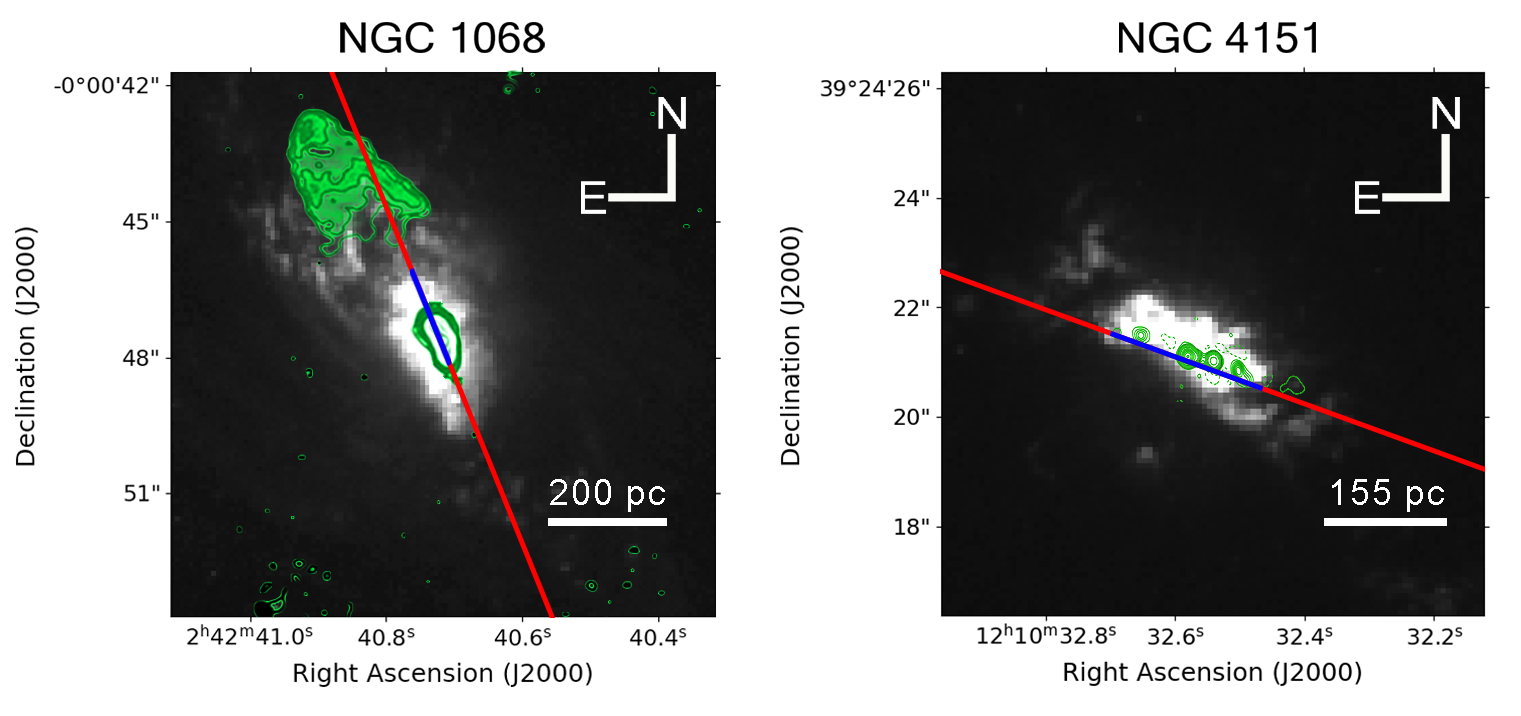
\includegraphics[width=1\linewidth]{figures/observations_and_data_reduction/seyferts_wfpc2.png}
    \caption[The slit positions of the archival HST/STIS observations plotted over archival {[}OIII{]} and radio-continuum imaging of NGC\;1068 and NGC\;4151.]{The slits of the archival STIS observations (red) shown plotted over archival HST/WFPC2 [OIII] emission-line images of the inner regions of NGC\;1068 and NGC\;4151, taken with the F502N filter (NGC\;1068: GTO:5754, PI Ford; NGC\;4151: GTO:5124; PI Ford). The spatial extents of the regions considered in this study (the extracted apertures: Section\;\ref{section: stis_seyferts: apertures}) along the slits are shown in blue. \textbf{Left:} The STIS slit shown over the [OIII] emission-line image of the near-nuclear regions of NGC\;1068; VLA 22\;GHz contours from \citet{Gallimore1996} are presented in green, showing the radio structure near the core and an extended lobe to the NE. \textbf{Right:} the STIS slit shown over the [OIII] emission-line image of the near-nuclear regions of NGC\;4151; the green contours are from high-resolution e-MERLIN 1.5\;GHz imaging presented by \citet{Williams2017}, and show a string of radio knots near the nucleus. I note that, while the narrow-band images are not continuum-subtracted, the brighter parts of the NLR emission are dominated by [OIII] emission in the filter bandpass, and so the images provide a good representation of the main NLR structures.}
    \label{fig: observations_and_data_reduction: stis_seyferts: observations: seyferts_wfpc2}
\end{figure*}

\subsection{Reduction of STIS data}
\label{section: stis_seyferts: observations_and_data_reduction data_reduction}

The first step in the data reduction was performed with the standard \mbox{\textsc{CALSTIS}} pipeline. For NGC\;1068, only a single exposure for each grating was available, while for NGC\;4151 I took the average of two exposures for each grating using \textsc{Python} scripts which made use of the \textsc{Numpy} \citep{Harris2020} and \mbox{\textsc{AstroPy}} \citep{AstropyCollaboration2013, AstropyCollaboration2018} modules. In order to ensure that the individual exposures for each grating were aligned, spatial slices were first extracted along the slit direction in a line-free region of the continuum covering the wavelength range 5480--5600\;{\AA} for the G430L grating and 6795--6890\;{\AA} for the G750L grating. The centroids of the spatial peaks --- determined with Gaussian-profile fits --- were consistent within 0.4\;pixels, confirming that each exposure was taken with the same telescope pointing within 0.02\;arcseconds. I also verified that the spectra taken with the G430L and G750L gratings for each object were aligned, using the same method of Gaussian-profile fits to the spatial flux profiles. Again, the spatial positions of the peak flux between gratings were consistent to within 0.4\;pixels, indicating that the observations with different gratings were closely spatially aligned.

Residual hot pixels and cosmic rays were removed from the spectra using the \textsc{CLEAN} command of the \textsc{STARLINK FIGARO} software package \citep{Currie2014}. Galactic-extinction correction was performed in the same manner as that done for IC\;5063 (Section\;\ref{section: xshooter_ic_5063: observations_and_data_reduction: data_reduction}) --- from the S98 and SF11 maps, the mean colour excesses in the directions of NGC\;1068 and NGC\;4151 were found to be \mbox{E(B-V)$_\mathrm{mean}=0.0289\pm0.0004$} and \mbox{E(B-V)$_\mathrm{mean}=0.0237\pm0.0011$}, respectively, and these values were used with the CCM89 $R_\mathrm{v}=3.1$ extinction law to correct for Galactic extinction.

\subsection{Aperture selection and extraction}
\label{section: stis_seyferts: apertures}

The reduced STIS long-slit spectra of NGC\;1068 and NGC\;4151 show disturbed kinematics (indicating outflows) and several bright emission-line knots in the central few hundred parsecs, as noted by previous studies \citep{Crenshaw2000a, Kraemer2000II, Das2005, Das2006, Meena2023}. Several apertures (integrated groupings of pixel rows) were extracted from the two-dimensional G430L and G750L spectra, following the methodology described in Section\;\ref{section: xshooter_ic_5063: observations_and_data_reduction: apertures}. Each aperture formed an integrated one-dimensional spectrum that corresponds to a certain spatial position along the slit, the locations of which were chosen to cover the locations of the bright emission knots seen in the two-dimensional spectra (Figure\;\ref{fig: stis_seyferts: apertures}). The widths of the apertures (6--15\;pixels; 0.3--0.8\;arcseconds) were set to contain sufficient signal in the emission lines that are used for diagnostics in this analysis, namely the fainter transauroral [OII]$\lambda\lambda$7319,7331 and [SII]$\lambda\lambda$4068,4076 doublets. The same apertures were extracted from the G430L and G750L spectra for each object, as it was previously determined that the spectra were closely spatially aligned. Flux errors were determined by adding the flux errors from individual pixel rows (which constitute a given aperture) in quadrature. As an example, part of the spectrum of Aperture 2 for NGC\;1068 is presented in Figure\;\ref{fig: stis_seyferts: ngc1068_g430l_ap2}. The chosen apertures extended to a maximum radial distance of 139\;pc for NGC\;1068, and 151\;pc in the case of NGC\;4151.

\begin{figure*}[!ht]
	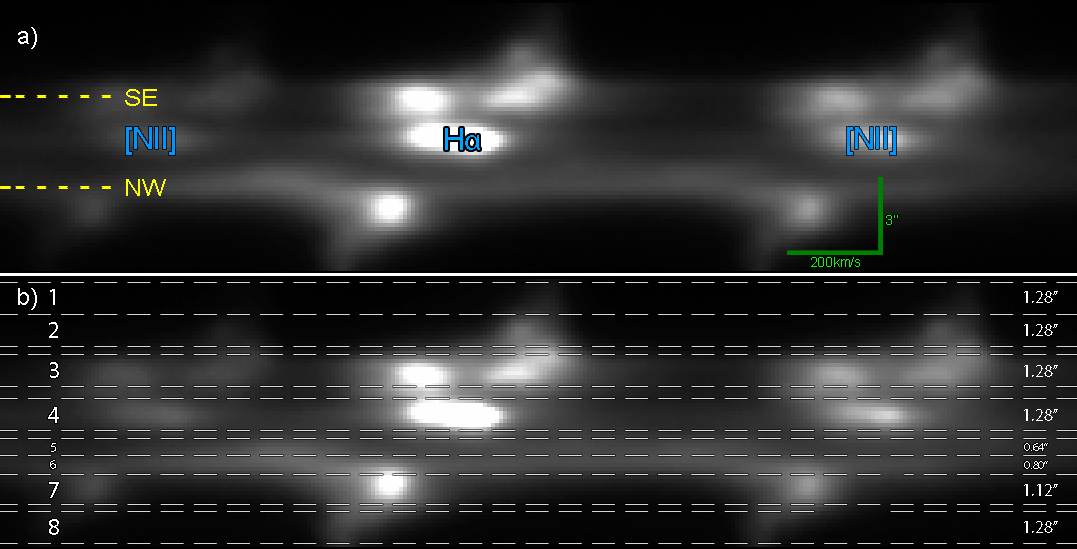
\includegraphics[width=\linewidth, trim={-3.8cm 0 0 0}, clip]{figures/stis_seyferts/apertures.png}
	\caption[Long-slit spectra of NGC\;1068 and NGC\;4151, with the positions and sizes of extracted apertures overlaid.]{Apertures for NGC\;1068 (left) and NGC\;4151 (right), positioned over the [OIII]$\lambda\lambda$4959,5007 doublet in the two-dimensional STIS G430L spectra. The spectral direction is horizontal (left = bluewards; right = redwards) and the vertical direction is spatial along the slit (with the direction shown by the labelled arrows); velocity scale bars are shown in green, and spatial scale bars are shown to the right of each spectrum. The apertures are shown as regions bounded by dashed lines, and are labelled on the left of each image --- they were chosen to contain enough signal for the measurement of faint lines in distinct kinematic regions within the central few hundred parsecs of each galaxy.}
	\label{fig: stis_seyferts: apertures}
\end{figure*}

Aperture 3 for NGC\;1068 was placed over a bright emission knot that corresponds to a previously-detected radio source at the likely position of the galaxy's nucleus (see discussion in \citealt{Kraemer2000II}), while Aperture 4 for NGC\;4151 corresponds to the location along the slit that is closest to the nucleus. Note that the spectra for NGC\;4151 do not directly cover the nucleus due to the 0.1\;arcsecond slit offset to the south that was performed to avoid nuclear contamination. Unfortunately, the south-west part of the slit for NGC\;1068 (seen above Aperture 4 in Figure\;\ref{fig: stis_seyferts: apertures}) did not contain enough signal for the measurement of the faint [OII]$\lambda\lambda7319,7331$ transauroral doublet, even when integrated as a single aperture. Therefore, this region is omitted from any analysis. 

\begin{figure*}[!ht]
    \centering
    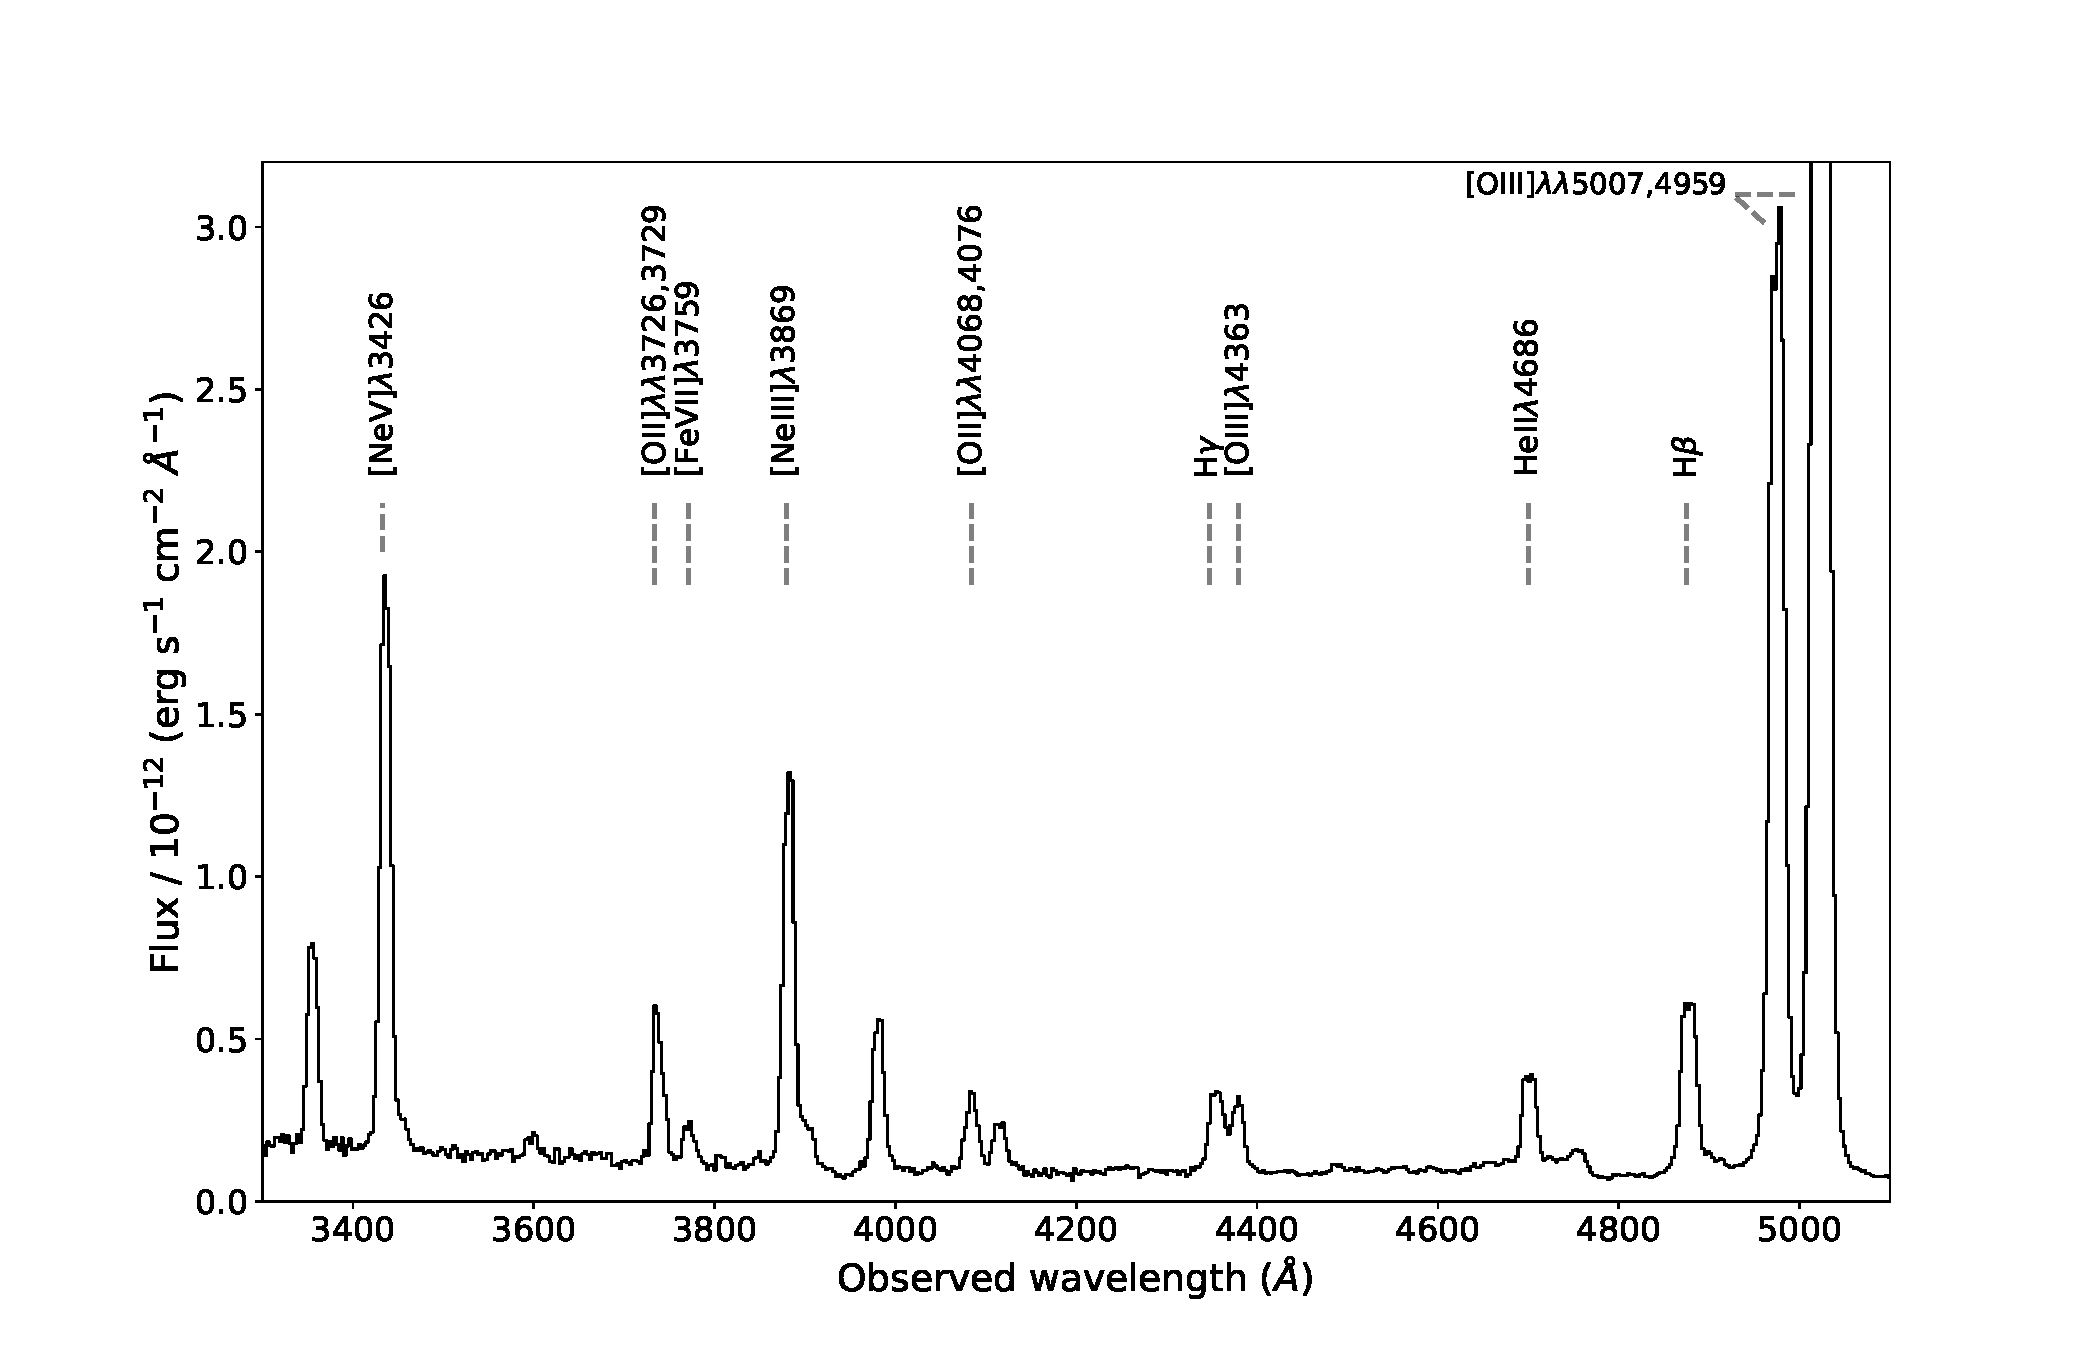
\includegraphics[width=\linewidth]{figures/stis_seyferts/ngc1068_g430l_ap2.pdf}
    \caption[HST/STIS G430L grating spectrum for Aperture 2 of NGC\;1068.]{The G430L grating spectrum for Aperture 2 of NGC\;1068 (Figure\;\ref{fig: stis_seyferts: apertures}). Key emission lines that are used in the analysis are labelled with dotted lines. Note that, for presentation reasons, the limit on the flux axis has been chosen so that fainter lines can be seen clearly; as a result, the peak of the [OIII]$\lambda$5007 line is not visible.}
    \label{fig: stis_seyferts: ngc1068_g430l_ap2}
\end{figure*}

Following aperture extraction, I ensured that the flux calibration was consistent between the two gratings for each aperture by overplotting the spectra in the region where the wavelength ranges of the gratings overlap (5275--5705\;{\AA}). It was found that all apertures for NGC\;1068 are closely matched in flux. However, for apertures 2 and 4 of NGC\;4151, the flux in the overlap region was \textgreater8\;per cent higher in the G430L grating than the G750L grating, potentially due to internal reflections within the instrument caused by the bright Type 1 nucleus (see \citealt{Nelson2000}). Therefore, these apertures are not used in further analysis. 

\subsection{The contribution of stellar continua to the spectra}
\label{section: stis_seyferts: stellar_continua}

The underlying stellar continua in NGC\;1068 and NGC\;4151 were not modelled and subtracted (as was done for IC\;5063: Section\;\ref{section: xshooter_ic_5063: observations_and_data_reduction: starlight}) for various reasons. First, the archival STIS G430L and G750L spectra did not have sufficient spectral resolution to clearly resolve absorption features that could be used to verify the robustness of the continuum fits. Second, there may be substantial contamination by direct and scattered AGN continuum \citep{Antonucci1985} and nebular continuum \citep{Tadhunter2016} that precludes accurate stellar-continuum modelling. Finally, the emission lines in the spectra have relatively-high equivalent widths, which fill in various stellar absorption features.

In order to verify whether stellar-continuum modelling was needed in this study, equivalent widths (EWs) for the H$\mathrm{\beta}$ recombination line were measured. Equivalent widths in the range \mbox{36\;\textless\;EW\;\textless\;148\;{\AA}} were found for the NGC\;1068 apertures and \mbox{30\;\textless\;EW\;\textless\;151\;{\AA}} for the NGC\;4151 apertures. The lowest measured emission-line equivalent width ($\mathrm{EW}=30$\;{\AA} for Aperture 3 in NGC\;4151) is a factor of three higher than that of the H$\mathrm{\beta}$ absorption feature as modelled for a $\sim$400\;Myr old stellar population (which gives the highest EWs in modelling by \citealt{GonzalezDelgado1999}). Thus, underlying stellar-absorption features may affect the H$\mathrm{\beta}$ luminosities measured in this work by a maximum factor of 1.3 (for a stellar $\mathrm{EW}=10$\;{\AA}). However, this is very much an upper limit since there is no clear Balmer break in the continua in any of the apertures, as would be expected for intermediate-age stellar populations that have strong Balmer absorption lines.

\subsection{Fits to key emission lines}
\label{section: stis_seyferts: oiii_models}

The NLR kinematics in NGC\;1068 and NGC\;4151 are complex, and have been previously modelled in detail as biconical outflows based on higher-resolution STIS spectra than those used here (\citealt{Das2006} and \citealt{Das2005} respectively; but see also \citealt{Crenshaw2000_N1068} and \citealt{Crenshaw2000_N4151}). In those studies, the [OIII]$\lambda\lambda$4959,5007 doublet line-profiles were fit with multiple Gaussian components for each pixel row of the two-dimensional spectra. Here, a similar procedure is performed for the extracted apertures by simultaneously fitting a first- or second-order polynomial to the continuum surrounding the [OIII]$\lambda\lambda$4959,5007 doublet, in addition to one or two Gaussian profiles to each of the lines within the doublet itself. The wavelength separation of the lines in the doublet, as well as the intensity ratio of the lines ($1:2.99$), were set to those defined by atomic physics \citep{Osterbrock2006}. Furthermore, the widths of a given Gaussian component were constrained to be the same for each line in the doublet. The resulting model parameters for each aperture are presented in Table \ref{tab: oiii_models}.

The difference between the mean wavelength of each Gaussian component and the rest [OIII] wavelength in the reference frame of the galaxy was calculated using redshifts\footnote{21\;cm redshifts from the NASA/IPAC Extragalactic Database (\url{https://ned.ipac.caltech.edu/}).} of $z=0.00381$ for NGC\;1068 and $z=0.003262$ for NGC\;4151. The intrinsic width of each component was also determined by subtracting the instrumental width of the STIS G430L grating in quadrature from the measured widths. According to the STIS manual, for a slit of width 0.1\;arcseconds, the instrumental broadening in the spectral direction is in the range \mbox{2\;\textless\;FWHM\;\textless\;3} pixels, corresponding to \mbox{5.5\;\textless\;FWHM\;\textless\;8.2\;{\AA}} for the G430L grating and \mbox{9.8\;\textless\;FWHM\;\textless\;14.8\;{\AA}} for the G750L grating. By fitting single Gaussian profiles to the [OIII]$\lambda\lambda$4959,5007 emission-line doublet at a radial distance of 4\;arcseconds from the nucleus of NGC\;4151 in the G430L spectra (where the lowest line widths are measured), a line width of FWHM$_\mathrm{inst}=6.0\pm0.4$\;{\AA} was measured; similarly, measuring the [SII]$\lambda$9531 line in the G750L spectra with this method resulted in a line width of FWHM$_\mathrm{inst}=12.3\pm2.4$\;{\AA}. Thus, instrumental widths of FWHM$_\mathrm{inst}=6.0$\;{\AA} (360\;km\;s$^{-1}$ at 5007\;{\AA}) and FWHM$_\mathrm{inst}=12.3$\;{\AA} (560\;km\;s$^{-1}$ at 6575\;{\AA}) are adopted here for the G430L and G750L gratings, respectively.

In subsequent analysis, only \textit{total} line fluxes --- including all Gaussian components used --- are considered, rather than fluxes from individual components (i.e. potentially representing outflowing and quiescent gas). This was done because the low spectral resolutions of the G430L and G750L gratings made it challenging to separate different kinematic components in cases where lines are heavily blended. Nonetheless, in order to improve the accuracy of the fits to the weaker emission lines and blends in the spectra, the kinematics (velocity shifts and widths) derived from fits to the [OIII] doublet in each aperture were used to constrain the fits to the other key diagnostic lines, such as H$\mathrm{\beta}$, H$\mathrm{\gamma}$, [OIII]$\lambda$4363, [OII]$\lambda$3726,3729, [OII]$\lambda\lambda$7319,7331, [SII]$\lambda\lambda$4068,4076, [SII]$\lambda\lambda$6717,6731, [ArIV]$\lambda\lambda$4711,4740 and HeII$\lambda$4686. It was found that this procedure produced acceptable fits to these lines, including the transauroral [SII]$\lambda\lambda$4068,4076 and [OII]$\lambda\lambda$7319,7331 doublets. However, for closely spaced doublets such as [OII]$\lambda$3726,3729, the low spectral resolution meant that individual lines were not resolved, and so the \textit{total} doublet profile was modelled as a single emission line during the fitting process.

\begin{table*}
    \def\arraystretch{1.2}
    \centering
    \begin{tabular}{lcccccc}
    \multirow{2}{*}{Aperture} & Distance & Distance  & $v_\mathrm{c, a}$ & FWHM$_\mathrm{c, a}$ & $v_\mathrm{c, b}$ & FWHM$_\mathrm{c, b}$ \\ 
        & (arcseconds) & (pc) & (km\;s$^{-1}$) & (km\;s$^{-1}$) & (km\;s$^{-1}$) & (km\;s$^{-1}$) \\
    \multicolumn{7}{c}{\vspace{-0.4cm}} \\
    \multicolumn{7}{c}{NGC 1068} \\ \hline
    1 & $-1.45$ & $-97$ & $-828\pm$4 & 572$\pm$25 & 295$\pm$40 & 1078$\pm$96 \\
    2 & $-0.74$ & $-50$ & $-184\pm$7 & 1017$\pm$31 & --- & --- \\
    3 & $-0.23$ & $-15$ & $-306\pm$3 & 662$\pm$26 & $-5\pm$20 & 1770$\pm$43 \\
    4 & $0.10$ & $7$ & $95\pm$3 & 367$\pm$26 & 235$\pm$8 & 1684$\pm$34 \\
    \multicolumn{7}{c}{\vspace{-0.4cm}} \\
    \multicolumn{7}{c}{NGC 4151} \\ \hline
    1 & $-1.58$ & $-123$ & $-172\pm$2 & 420$\pm$25 & $-263\pm$29 & 1261$\pm$102 \\
    3 & $-0.38$ & $-30$ & $-392\pm$6 & 0$\pm28$\;$^a$ & $-356\pm$3 & 1065$\pm$26 \\
    5 & 0.48 & $37$ & $34\pm$1 & 234$\pm$24 & 121$\pm$11 & 1013$\pm$44 \\
    6 & 1.02 & $80$ & $40\pm$1 & 307$\pm$25 & 126$\pm$8 & 768$\pm$35 \\
    \end{tabular} \\
    \vspace{12pt}
    $^a$ The measured width of the \textit{component} is consistent with the instrumental width, and hence unresolved. \\
    \caption[{[}OIII{]} model parameters and aperture distances for each of the apertures for NGC\;1068 and NGC\;4151.]{[OIII] model parameters (galaxy rest-frame component velocity shift: $v_\mathrm{c}$; instrumentally-corrected component velocity width: FWHM$_{c}$) and distances from the nucleus (in arcseconds and pc) for each of the apertures for NGC\;1068 and NGC\;4151. In apertures where there are multiple Gaussian components for the [OIII] models, the kinematic parameters for the two components are labelled with the subscripts `a' and `b'.}
    \label{tab: oiii_models}
\end{table*}

\section{Analysis of the STIS spectra}
\label{section: stis_seyferts: analysis}

\subsection{Transauroral-line diagnostics}
\label{section: stis_seyferts: tr_diagnostics}

In order to provide estimates of the electron densities of the warm-ionised gas in NGC\;1068 and NGC\;4151, I made use of the transauroral-line-ratio technique (first described by \citealt{Holt2011}) that was verified and used in Chapter \ref{chapter: xshooter_ic5063}, for two key reasons. First, these lines have sufficiently-high critical densities (Appendix \ref{appendix: properties_of_warm_ionised_diagnostic_lines}) to be sensitive to the electron density values that have previously been determined for these objects ($10^{3.0}$\;\textless\;$n_e$\;\textless\;$10^{7.2}$\;cm$^{-3}$). Second, because the transauroral-line method uses the ratios of the \textit{total} line fluxes of widely-separated emission-line doublets (unlike the commonly-used [OII](3726/3729) and [SII](6717/6731) ratios), this method is less susceptible to uncertainties from fit degeneracy resulting from the larger velocity widths (as is often the case for outflowing gas) and low spectral resolutions (as for the G430L and G750L STIS gratings) that lead to the blending of line profiles within the doublets. 

\newpage
The [OIII] models were fit to the transauroral lines to measure line fluxes, which were then used to calculate the TR ratios
\begin{align*}
TR([OII]) = F(3726 + 3729) / F(7319 + 7331), \\
TR([SII]) = F(4068 + 4076) / F(6717 + 6731).
\end{align*} 
As in Chapter \ref{chapter: xshooter_ic5063}, the \textsc{CLOUDY} code (version C17.02: \citealt{Ferland2017}) was used to generate plane-parallel, single-slab, radiation-bounded models of solar-composition gas with no dust depletion, photoionised by a central source. The ionising continuum of this source followed a power-law of shape $F_v \propto v^{-\alpha}$ between 10\;{\textmu}m and 50\;keV, with a spectral index of $\alpha=1.5$. I note, however, that the TR ratios are relatively insensitive to the shape of the ionising continuum (see Appendix B in \citealt{Santoro2020}). The ionisation parameter was set to log\;$U=-3$ (the highest value that reproduced the measured TR ratios), and the electron density of the modelled gas was varied in 0.01\;dex steps between \mbox{2.00\;\textless\;log$_{10}(n_e$ [cm$^{-3}$])\;\textless\;5.00}. The modelled TR ratios produced for each electron density value were then reddened with the $R_\mathrm{v}=3.1$ CCM89 law, producing a grid of values that could be compared to the measured ratios in order to provide simultaneous determinations of electron density and reddening. The resulting TR grid is shown in Figure\;\ref{fig: stis_seyferts: tr_ddd}, and the derived values are given in Table {\ref{tab: stis_seyferts: ne_ebv_te}}.

\begin{table*}
    \def\arraystretch{1.4}
    \centering
    \begin{tabular}{lccc}
    Aperture & log$_{10}(n_e$[cm$^{-3}$]) & E(B-V)$_\mathrm{TR}$ & $T_e$ (K) \\ 
    \multicolumn{4}{c}{\vspace{-0.4cm}} \\
    \multicolumn{4}{c}{NGC\;1068} \\ 
    \hline
    1 & 4.06$^{+0.05}_{-0.06}$ & 0.16$^{+0.04}_{-0.05}$ & 14300$^{+2100}_{-1300}$ \\
    2 & 4.65$^{+0.05}_{-0.04}$ & 0.05$^{+0.04}_{-0.05}$ & 14400$^{+1500}_{-1100}$ \\
    3 & 4.74$^{+0.05}_{-0.05}$ & 0.16$^{+0.05}_{-0.04}$ & 16100$^{+1400}_{-1000}$ \\
    4 & 4.45$^{+0.09}_{-0.09}$ & 0.17$^{+0.08}_{-0.08}$ & 16000$^{+1600}_{-1100}$ \\
    \multicolumn{4}{c}{\vspace{-0.4cm}} \\
    \multicolumn{4}{c}{NGC\;4151} \\ 
    \hline
    1 & 3.68$^{+0.08}_{-0.10}$ & 0.11$^{+0.05}_{-0.07}$ & 16300$^{+3400}_{-1800}$ \\
    3 & 4.04$^{+0.07}_{-0.15}$ & 0.13$^{+0.05}_{-0.06}$ & 21000$^{+3300}_{-2100}$ \\
    5 & 3.94$^{+0.10}_{-0.10}$ & 0.15$^{+0.08}_{-0.08}$ & 17300$^{+5200}_{-2400}$ \\
    6 & 3.75$^{+0.8}_{-0.10}$  & 0.23$^{+0.07}_{-0.07}$ & 15200$^{+3400}_{-1800}$ \\
    \end{tabular}
    \caption[Electron densities, reddening values, and electron temperatures for NGC\;1068 and NGC\;4151.]{Electron densities, reddening values and electron temperatures for the NGC\;1068 and NGC\;4151 apertures. The densities and reddenings were determined simultaneously using the transauroral-line technique (Section\;\ref{section: stis_seyferts: tr_diagnostics}; Figure\;\ref{fig: stis_seyferts: tr_ddd}), and the temperatures were determined using the [OIII](5007+4959)/4363 ratio (Section\;\ref{section: stis_seyferts: electron_temperatures}).}
    \label{tab: stis_seyferts: ne_ebv_te}
\end{table*}

The electron densities measured in this way for NGC\;1068 have values in the range \mbox{4.00\;\textless\;log$_{10}(n_e$\;[cm$^{-3}$])\;\textless\;4.75}, while those for NGC\;4151 are approximately an order of magnitude lower (\mbox{3.60\;\textless\;log$_{10}(n_e$\;[cm$^{-3}$])\;\textless\;4.10}). This is the first time that densities above $n_e=10^{3.5}$\;cm$^{-3}$ have been found using the transauroral lines with \textit{spatially-resolved} observations; these values agree with similarly high electron densities derived using this technique for non-spatially resolved observations of other AGN (e.g. \citealt{Holt2011, Rose2018, Santoro2018, Spence2018, Davies2020, Speranza2022}). Importantly, the densities found here are above the upper sensitivity limit of the traditional [OII](3726/3729) and [SII](6717/6731) line ratios (Appendix \ref{appendix: properties_of_warm_ionised_diagnostic_lines}), and since broad (outflowing) and narrow (quiescent; non-outflowing) components are not separated, are likely to be underestimates for the outflowing gas (which is expected to be denser than the quiescent gas: e.g. \citealt{VillarMartin1999}; Chapter \ref{chapter: xshooter_ic5063}). The reddening values that are measured are relatively modest, and in the range \mbox{0.05\;\textless\;E(B-V)$_\mathrm{TR}$\;\textless\;0.25} for both objects --- these values were used to deredden the spectra for all further analysis.

\begin{figure}[!t]
    \centering
    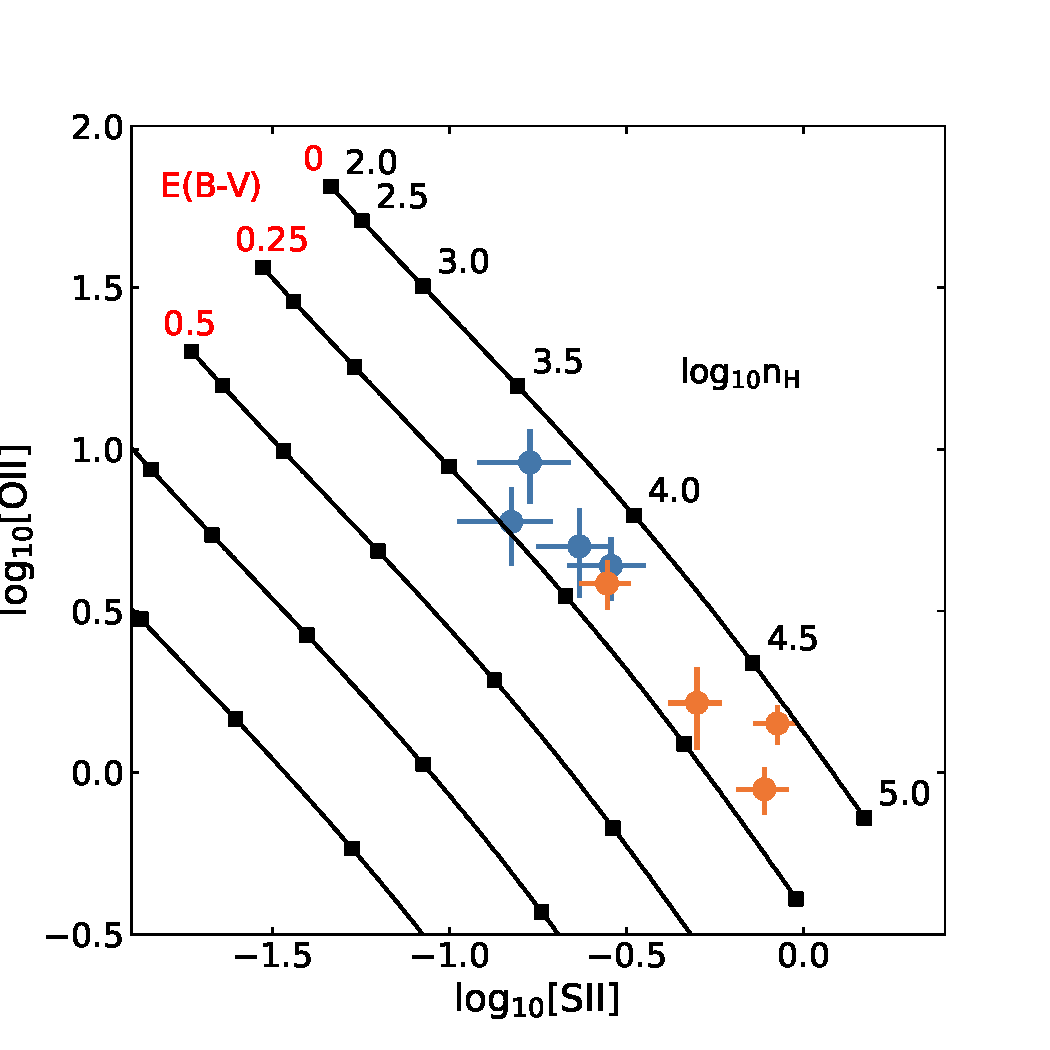
\includegraphics[width=0.8\linewidth]{figures/stis_seyferts/tr_ddd_seyferts.pdf}
    \caption[Transauroral {[}OII{]} and {[}SII{]} line ratio diagram for NGC\;1068 and NGC\;4151, showing both measured values and those predicted from photoionisation modelling.]{Grid of modelled transauroral (TR) [SII] and [OII] line ratios for radiation-bounded gas at different electron densities and reddenings (black joined squares; as modelled with the \textsc{Cloudy} code and the CCM89 extinction curve), and measured line ratios for the NGC\;1068 (orange circles) and NGC\;4151 (blue circles) apertures.}
    \label{fig: stis_seyferts: tr_ddd}
\end{figure}

\subsection{Ionisation states and mechanisms of the warm-ionised gas}
\label{section: stis_seyferts: mechanisms}

The relatively-low-ionisation transauroral lines must be emitted by radiation-bounded clouds --- therefore, it is uncertain how well densities derived from the transauroral ratios would represent the densities of clouds or cloud complexes that have been shock-ionised or have significant matter-bounded components. Furthermore, the model used in the transauroral-ratio method assumes radiation-bounded AGN-photoionised clouds, with no contribution from a matter-bounded component or shock-ionisation. Similarly, the multi-component ionisation modelling by \citet{Revalski2021} --- which has previously been applied to NGC\;1068 and NGC\;4151 --- uses AGN-photoionisation models. Therefore, it is important to investigate the ionisation mechanisms for the gas detected in the STIS slits, which potentially can also give information regarding the outflow acceleration mechanism(s) present.

\subsubsection{Electron temperatures}
\label{section: stis_seyferts: electron_temperatures}

Electron temperatures of the warm ionised phase are expected to be higher for shocked gas than AGN-photoionised gas (e.g. \citealt{Fosbury1978, VillarMartin1999}). Therefore, to provide a first indication of the ionisation mechanisms of the warm-ionised gas observed in the apertures, electron temperatures were measured using the (dereddened) [OIII](5007+4959)/4363 emission-line ratio and the \textsc{PyNeb Python} module \citep{Luridiana2015}, taking the electron densities for the apertures to be those derived using the transauroral-line technique for both objects (3.75\;\textless\;log$_{10}(n_e$\;[cm$^{-3}$])\;\textless\;4.75: see Table\;\ref{tab: stis_seyferts: ne_ebv_te} and Section\;\ref{section: stis_seyferts: tr_diagnostics}). Electron temperatures measured in this way are presented in Table\;\ref{tab: stis_seyferts: ne_ebv_te} --- values in the range $14,300$\;\textless\;$T_e$\;\textless\;$21,000$\;K are found for every aperture in both objects, with the highest temperatures (up to $T_e=21,000$\;K) being found in the central apertures of NGC\;4151. These high electron temperatures may not be fully explainable as being due to AGN-photoionisation of radiation-bounded gas (\citealt{Fosbury1978, Binette1996, VillarMartin1999}; Chapter \ref{chapter: xshooter_ic5063}).

\subsubsection{Shock-ionisation vs matter-bounded AGN-photoionisation}
\label{section: stis_seyferts: shock_vs_agn}

In order to investigate the cause of the high electron temperatures further, the [OIII](5007/4363) vs HeII/H$\mathrm{\beta}$ diagnostic diagram (developed by \citealt{VillarMartin1999}) was produced for the apertures for NGC\;1068 and NGC\;4151 --- this is shown in Figure\;\ref{fig: stis_seyferts: oiii_heii_hbeta_stis}. The radiation-bounded photoionisation models shown here are the same as those used for the TR ratio grid in Section\;\ref{section: stis_seyferts: tr_diagnostics} (Figure\;\ref{fig: stis_seyferts: tr_ddd}), albeit for an electron density of $n_e=10^{4}$\;cm$^{-3}$, varying ionisation parameters (between $-3.5$\;\textless\;log$_{10}U$\;\textless\;$-2.0$), and two values of spectral index ($\alpha=1.0$, 1.5)\footnote{The effect of varying the photoionisation model parameters on the [OIII](5007/4363) vs HeII/H$\mathrm{\beta}$ diagnostic diagram is investigated in Appendix \ref{appendix: heii_hb_oiii_photoionisation_modelling}.}. The pure-shock and precursor (pre-shock) models are taken from the \textsc{MAPPINGS III} library presented by \citet{Allen2008}, with varying shock velocities in the range 100\;\textless\;$v_\mathrm{shock}$\;\textless\;1000\;km\;s$^{-1}$ and magnetic parameters of \mbox{$B/\sqrt{n}$ = 2,4\;$\mu$G\;cm$^{3/2}$} for a solar-composition pre-shock gas with a density of \mbox{$n$ = 10$^{2}$\;cm$^{-3}$}. The magnetic parameters were chosen to cover a reasonable range of values expected in the ISM \citep{Dopita1995}, in addition to being close to the magnetic parameters near equipartition (\mbox{$B/\sqrt{n}\sim3.23\;\mu$G\;cm$^{3/2}$}: \citealt{Allen2008}). Note that, as in Chapter \ref{chapter: xshooter_ic5063}, the standard `BPT' diagrams \citep{Baldwin1981} are not used here to investigate the ionisation of the gas because the regions of photo- and shock-ionisation in those diagrams overlap considerably (see Section\;\ref{section: introduction: outflows: accleration_mechanisms: ionisation_and_excitation_mechanisms}, Figure\;\ref{fig: introduction: outflows: acceleration_mechanisms: bpt_diagram_photo_shock_ionisation}). Furthermore, some of the lines involved in those diagrams (such as H$\mathrm{\alpha}$ and [NII]$\lambda\lambda$6548,6583) are strongly blended in the apertures considered here due to the outflow kinematics and the relatively-low spectral resolution, and therefore are affected by major fit degeneracies.

In Figure\;\ref{fig: stis_seyferts: oiii_heii_hbeta_stis}, the [OIII](5007/4363) and HeII/H$\mathrm{\beta}$ line ratios are also plotted as functions of A$_\mathrm{M/I}$: the ratio of the solid angles subtended by matter-bounded clouds and radiation-bounded clouds, from modelling by \citet{Binette1996}. This ratio allows estimations of the relative contribution of matter-bounded clouds and radiation-bounded clouds in the apertures. The modelling by \citet{Binette1996} assumes solar-metallicity gas, with an ionising-source spectral index of $\alpha=-1.3$, an ionisation parameter of log\;$U=-1.4$, and a density of $n_\mathrm{MB}=50$\;cm$^{-3}$. In this model, the radiation-bounded clouds are ionised by UV photons which have passed through the matter-bounded component, thus the shape of the ionising spectrum reaching the radiation-bounded clouds has changed relative to that from the source --- the parameters of the radiation-bounded clouds are determined using the resulting ionising spectrum and by assuming that the clouds have fixed pressures.

Due to line-blending effects and the continuum underlying the H$\mathrm{\beta}$, [HeII]$\lambda$4686, and [OIII]$\lambda$4363 lines being more complex than that which underlies the [OIII]$\lambda\lambda$4959,5007 doublet and transauroral lines, an MCMC (Markov Chain Monte Carlo) fitting routine was used to fit the lines involved in the HeII$\lambda$4686/H$\mathrm{\beta}$ and [OIII](5007/4363) ratios in each aperture for both objects --- this was done to ensure that line-flux uncertainties were not significantly overestimated due to the blending of spectral lines and the continuum. The results of the Gaussian fits described in Section\;\ref{section: stis_seyferts: oiii_models} (determined using least-squares optimisation) to these lines were used as initial starting points for the MCMC routine, which fit the same models (namely one or two Gaussian components and a low-order polynomial) to the spectra --- taking into account the flux uncertainty of the HST data --- with priors chosen to ensure that the resulting models were physical (i.e. the line fluxes, mean wavelengths, and line widths must have been positive). For each fit, 500 walkers were initialised in a Gaussian distribution around the starting parameters, and 5000 iterations (including a 1000 iteration `burn-in' phase) were used. The MCMC fits themselves were run using the \textsc{emcee} \textsc{Python} module \citep{FormanMackey2013}.

\begin{figure}[!p]
    \centering
    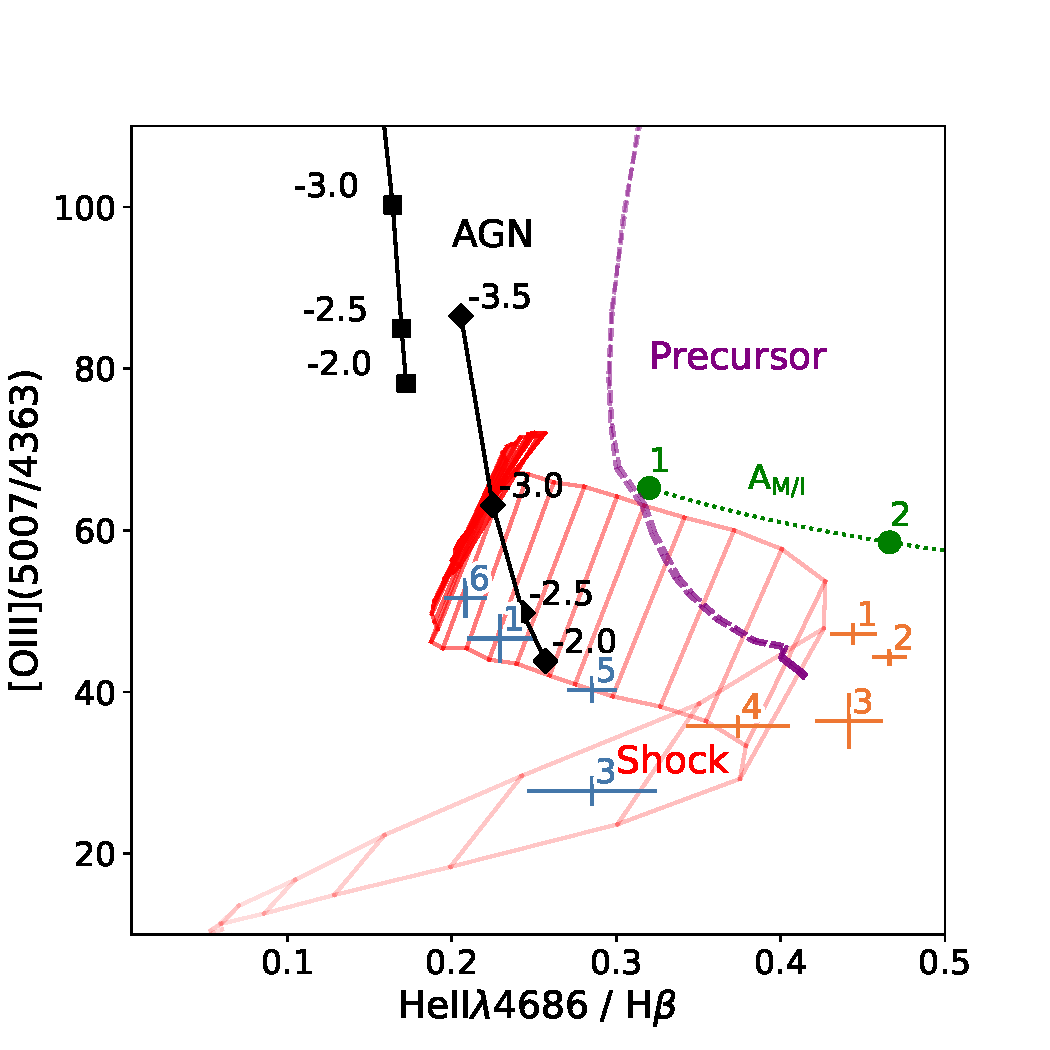
\includegraphics[width=0.8\linewidth]{figures/stis_seyferts/oiii_heii_hb_stis.pdf}
    \caption[HeII$\lambda$4686/H$\mathrm{\beta}$ vs {[}OIII{]}5007/{[}OIII{]}$\lambda$4363 diagnostic diagram for the warm-ionised gas in NGC\;1068 and NGC\;4151, including modelled values for (radiation-bounded and matter-bounded) photo- and shock-ionised gas.]{[OIII](5007/4363) vs HeII/H$\mathrm{\beta}$ diagnostic diagram \citep{VillarMartin1999}, used to distinguish between radiation-bounded AGN-photoionisation, matter-bounded AGN-photoionisation, and shock-ionisation. The black markers show the predicted line ratios from radiation-bounded \textsc{Cloudy} modelling (see Section\;\ref{section: stis_seyferts: tr_diagnostics}) for solar-composition gas with a density of \mbox{$n_e=10^{4}$\;cm$^{-3}$} and varying ionisation parameters (log\;$U$; labelled) and spectral indices (squares: $\alpha=1.5$; diamonds: $\alpha=1.0$). The solid red grid shows the line ratios predicted from shock modelling \citep{Allen2008} for solar-composition gas with a pre-shock density of \mbox{$n$ = 10$^{2}$\;cm$^{-3}$} and magnetic parameters of \mbox{$B/\sqrt{n}=2,4$\;$\mu$G\;cm$^{3/2}$}, with lighter regions on the plot corresponding to lower shock velocities. The purple dashed lines show the predicted emission from the precursor gas, which has not yet passed through (but is photoionised by) the shock, and the dotted green line shows the line ratios expected for different ratios of matter-bounded and radiation-bounded clouds (A$_\mathrm{M/I}$, labelled and marked with green circles) from photoionisation modelling by \citet{Binette1996}. Observed line ratios for each aperture are shown in orange for NGC\;1068 and blue for NGC\;4151, with the aperture number annotated.}
    \label{fig: stis_seyferts: oiii_heii_hbeta_stis}
\end{figure}

From Figure\;\ref{fig: stis_seyferts: oiii_heii_hbeta_stis}, there is clear evidence for significant matter-bounded emission in apertures 1, 2, and 3 in NGC\;1068, implied by high electron temperatures and HeII/H$\mathrm{\beta}$\;\textgreater\;0.4 (similar ratio values were also measured by \citealt{Kraemer2000III}); the approximate ratio of matter-bounded to radiation-bounded clouds is A$_\mathrm{M/I}\sim2$. The difference between the [OIII](5007/4363) ratios measured in the NGC\;1068 apertures and those predicted from the \citet{Binette1996} modelling can be explained as the models only representing one combination of parameters: it is possible for matter-bounded clouds with different parameters to have similar [OIII](5007/4363) ratios to those found for NGC\;1068. Specifically, this ratio would be smaller for higher electron densities than the low density assumed by \citet{Binette1996}. Moreover, the presence of matter-bounded emission in these apertures is supported by the strength of high-ionisation coronal emission lines (E$_\mathrm{ion}$\;\textgreater\;100\;eV), such as [NeV]$\lambda$3426, [FeVII]$\lambda$3759, and [FeVII]$\lambda$6087, relative to lower-ionisation lines (such as [OIII]) in the STIS spectra. These and other high-ionisation lines were previously identified in the same dataset by \citet{Kraemer2000II}. For Aperture 4 of NGC\;1068 (centred slightly above the nucleus: Figure\;\ref{fig: stis_seyferts: apertures}), the  HeII/H$\mathrm{\beta}$ ratios are consistent with both matter-bounded AGN-photoionisation and shock-ionisation. 

\begin{figure}[!t]
\centering
    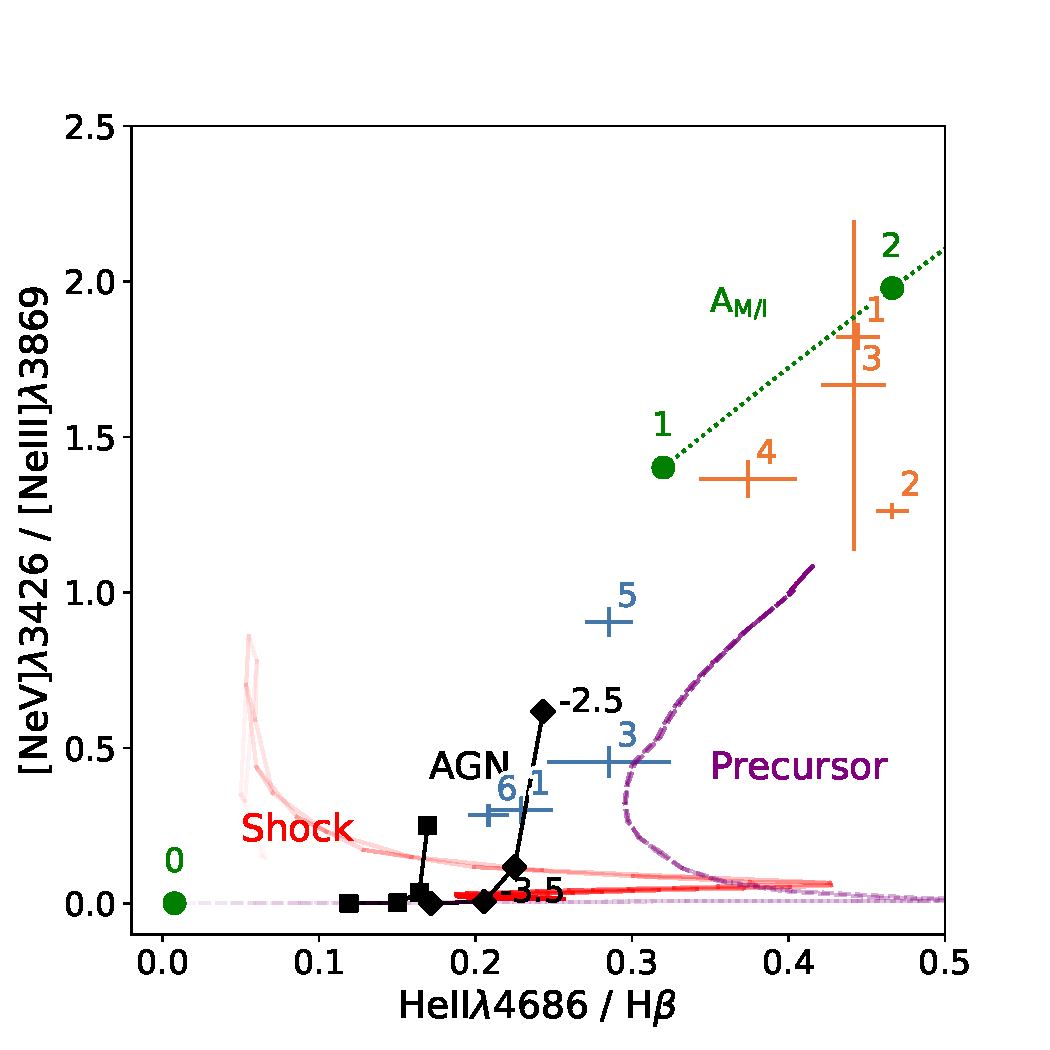
\includegraphics[width=0.8\linewidth]{figures/stis_seyferts/heii_nev_neii.pdf}
    \caption[{[}NeV{]}3426/{[}NeIII{]}3869 vs HeII/H$\mathrm{\beta}$ diagnostic diagram for the warm-ionised gas in NGC\;1068 and NGC\;4151, including modelled values for (radiation-bounded and matter-bounded) photo- and shock-ionised gas.]{[NeV]3426/[NeIII]3869 vs HeII/H$\mathrm{\beta}$ diagnostic diagram --- both ratios are sensitive to the presence of significant matter-bounded components. The line and marker scheme is the same as Figure\;\ref{fig: stis_seyferts: oiii_heii_hbeta_stis}. The line ratios measured in the NGC\;1068 apertures are located in the matter-bounded photoionisation region of the diagram (corresponding to \mbox{1\;\textless\;A$_\mathrm{M/I}$\;\textless\;2}; consistent with Figure\;\ref{fig: stis_seyferts:nev_neiii_heii_hbeta_stis}) whereas the NGC\;4151 line ratios fall in the shock/precursor/radiation-bounded AGN-photoionisation region.}
    \label{fig: stis_seyferts:nev_neiii_heii_hbeta_stis}
\end{figure}

To further probe the ionisation mechanism of the gas, the [NeV]$\lambda$3426/[NeIII]$\lambda$3869 ratio --- which is sensitive to higher-ionisation gas --- was also measured using the same MCMC fitting routine described earlier. A diagnostic diagram of [NeV]$\lambda$3426/[NeIII]$\lambda$3869 vs HeII/H$\mathrm{\beta}$ --- presented in Figure\;\ref{fig: stis_seyferts:nev_neiii_heii_hbeta_stis} --- was produced using the same radiation-bounded-photoionisation, matter-bounded-photoionisation, and shock-ionisation models as used for the [OIII](5007/4363) and HeII/H$\mathrm{\beta}$ diagram. It is found that the values for all of the NGC\;1068 apertures are consistent with matter-bounded AGN-photoionisation with  1\;\textless\;A$_\mathrm{M/I}$\;\textless\;2, further indicating that the gas in these apertures is matter-bounded and AGN-photoionised, including Aperture 4.

With the exception of Aperture 3, the [OIII](5007/4363) vs HeII/H$\mathrm{\beta}$ ratios measured in the NGC\;4151 apertures (Figure\;\ref{fig: stis_seyferts: oiii_heii_hbeta_stis}), are consistent with both shock-ionisation and radiation-bounded AGN-photoionisation (assuming a relatively flat spectral index of $\alpha=1.0$ and log\;$U\sim-2.0$). However, from the [NeV]$\lambda$3426/[NeIII]$\lambda$3869 vs HeII/H$\mathrm{\beta}$ diagram (Figure\;\ref{fig: stis_seyferts:nev_neiii_heii_hbeta_stis}), it can be seen that the measured ratios for NGC\;4151 are not consistent with pure shock-ionisation alone: if the gas is shock-ionised, then a contribution from the precursor component is required. Alternatively, the gas in these apertures may have pure radiation-bounded AGN-photoionisation, however, I highlight that this requires a relatively flat spectral index ($\alpha=1.0$), and/or higher ionisation parameters ($-3.0$\;\textless\;log\;$U$\;\textless\;$-2.0$) and densities ($n_e$\;\textgreater\;$10^5$\;cm$^{-3}$) than can explain the measured transauroral-line ratios (Section\;\ref{section: stis_seyferts: tr_diagnostics}). Ultimately, it is not possible to unambiguously determine the true, dominant ionisation mechanism of the gas in the NGC\;4151 apertures with the diagnostic features that are available in the STIS data.

\subsubsection{The viability of shock-ionisation}
\label{section: stis_seyferts: shock_viability}

In order to further investigate the viability of shocks as the dominant ionisation mechanism along the slits for NGC\;1068 and NGC\;4151, the measured H$\mathrm{\beta}$ fluxes were compared to those expected from shock models --- a technique presented by \citet{Baron2017}. First, I converted the measured (and dereddened) H$\mathrm{\beta}$ fluxes ($F_\mathrm{H\beta}$) into H$\mathrm{\beta}$ luminosities using the luminosity distance ($D_\mathrm{L}$) for each galaxy. The resulting luminosities were then converted into luminosities per surface area using the physical aperture sizes (i.e. the aperture width multiplied by the slit width). 

The measured luminosities per surface area were then compared to those expected from the \textsc{MAPPINGS III} shock models of pre-shock density $n=10^2$\;cm$^{-3}$ (corresponding to the densities measured in the apertures, assuming a compression factor of 100: \citealt{Sutherland2017}) and magnetic parameters $B/\sqrt{n}=2,4$\;$\mathrm{\mu}$G\;cm$^{3/2}$. From this comparison, it was found that the H$\mathrm{\beta}$ luminosities per surface area, as measured in each aperture for NGC\;1068 \mbox{($4.9\times10^{-3}$\;\textless\;L$_\mathrm{H\beta}$\;\textless\;$2.2\times10^{-2}$\;erg\;s$^{-1}$\;cm$^{-2}$)} and NGC\;4151 \mbox{($2.2\times10^{-3}$\;\textless\;L$_\mathrm{H\beta}$\;\textless\;$4.6\times10^{-3}$\;erg\;s$^{-1}$\;cm$^{-2}$)}, can be accounted for by shocks with velocities $v_\mathrm{shock}$\;\textgreater\;425\;km\;s$^{-1}$ and  $v_\mathrm{shock}$\;\textgreater\;225\;km\;s$^{-1}$ respectively. In both cases, the outflow velocities for the apertures (Section\;\ref{section: stis_seyferts: kinematics}; Table \ref{tab: energetics}) are above these required velocities. This demonstrates that shock-ionisation \textit{could} feasibly produce the recombination line fluxes measured in both objects, however, this alone does not necessarily confirm the ionisation mechanism.

I note that here a gas covering factor of unity relative to the shock (i.e. that the emitting gas covers the entire area of the shock within each aperture) is assumed, which may not be the case in reality. If this covering factor is in fact much lower than unity, then a larger shock area or higher shock velocities would be needed to produce the same $\mathrm{H\beta}$ luminosity.

\subsection{Electron densities of the high-ionisation gas in NGC 1068}
\label{section: stis_seyferts: high_ionisation}

The relative strengths of the high-ionisation (E$_\mathrm{ion}\gtrapprox100$\;eV) lines detected in several of the NGC\;1068 apertures indicate the presence of matter-bounded clouds, which may play an important role in the structure of the cloud complexes in the NLR. Determining the physical conditions of this high-ionisation component is therefore necessary. To this end, a diagnostic diagram consisting of the [FeVII](6087/3759) and [NeV]$\lambda$3426/[FeVII]$\lambda$6086 ratios (see \citealt{Rose2011}) was created (Figure\;\ref{fig: stis_seyferts: nev_fevii_a_vary}). The line fluxes involved in these ratios were determined using the same MCMC fitting method described in Section\;\ref{section: stis_seyferts: mechanisms}.

The ratios involved in the [FeVII](6086/3759) vs [NeV]$\lambda$3426/[FeVII]$\lambda$6086 diagnostic diagram are sensitive to both electron density and temperature, and thus the position of the AGN-photoionisation grid on this diagram changes with the assumed ionising-source spectral index ($\alpha$) and the ionisation parameter ($U$) of the gas. Therefore, the effect of varying spectral index, electron density, and ionisation parameter on this diagram was quantified before using it to derive electron densities. Two \textsc{CLOUDY} models for differing ionising-source spectral indices ($\alpha=1.0, 1.5$) were created (following the methodology described in Section\;\ref{section: stis_seyferts: high_ionisation}) for solar-metallicity, plane-parallel, single-slab clouds of varying ionisation parameters ($-3.5$\;\textless\;log\;$U$\;\textless\;2.0) and electron densities (5.0\;\textless\;log($n_e$\;[cm$^{-3}$])\;\textless\;8.0). The resulting line-ratio grids are presented on the [FeVII](6086/3759) vs [NeV]$\lambda$3426/[FeVII]$\lambda$6086 diagnostic diagram in Figure\;\ref{fig: stis_seyferts: nev_fevii_a_vary}, from which it can be seen that a flatter spectral index produces lower [NeV]$\lambda$3426/[FeVII]$\lambda$6086 ratios, with little effect on the [FeVII](6086/3759) ratios: for low values of [NeV]$\lambda$3426/[FeVII]$\lambda$6086 (i.e. as measured in Aperture 4 for NGC\;1068), the effect of this variation on derived density is small ($\sim$0.1\;dex). However, a shallower spectral index cannot reproduce higher values of [NeV]$\lambda$3426/[FeVII]$\lambda$6086 (as measured in NGC\;1068 apertures 2 and 3) without very low (log\;$U$\;\textless\;$-3.0$) ionisation parameters. Therefore, the \textsc{CLOUDY} grid with $\alpha=1.5$ was used to derive electron densities for the high-ionisation gas.

The measured line ratios for the NGC\;1068 apertures are plotted on the [FeVII](6086/3759) vs [NeV]$\lambda$3426/[FeVII]$\lambda$6086 diagram in Figure\;\ref{fig: stis_seyferts: nev_fevii_a_vary}. From the $\alpha=1.5$ grid, the densities of the high-ionisation gas were determined to be in the range 6.45\;\textless\;log$_{10}$($n_e$\;[cm$^{-3}$])\;\textless\;8.00: several orders of magnitude higher than the gas traced by the lower-critical-density [OII] and [SII] lines. The implications of this for the gas structures within the apertures are discussed in Section\;\ref{section: stis_seyferts: disc-density-mb}. 

\vspace*{\fill}

\begin{figure}[!ht]
    \centering
    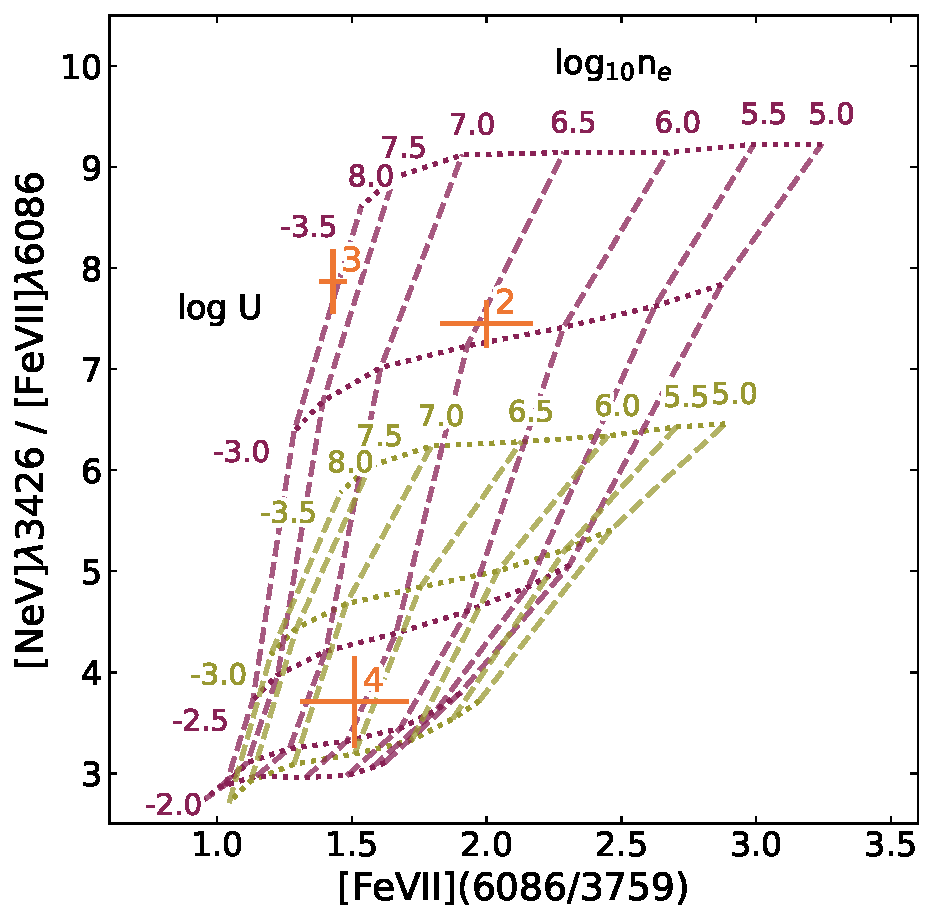
\includegraphics[width=0.7\linewidth]{figures/stis_seyferts/nev_fevii_vary_a.pdf}
    \caption[{[}FeVII{]}(6087/3759) vs {[}NeV{]}$\lambda$3426/{[}FeVII{]}$\lambda$6086 diagnostic diagram for the highly-ionised gas in NGC\;1068, along with grids produced from photoionisation modelling.]{[FeVII](6087/3759) vs [NeV]$\lambda$3426/[FeVII]$\lambda$6086 diagnostic diagram with radiation-bounded AGN-photoionisation grids generated with \textsc{CLOUDY} for two values of spectral index: $\alpha=1.0$ (green) and $\alpha=1.5$ (purple). Dashed lines connect points of constant density (labelled), and dotted lines connect points of constant ionisation parameter (also labelled). The measured ratio values in the NGC\;1068 apertures are shown in orange and labelled; from the $\alpha=1.5$ grid, the high-ionisation gas in NGC\;1068 is found to have densities in the range 6.45\;\textless\;log$_{10}$($n_e$\;[cm$^{-3}$])\;\textless\;8.00.}
    \label{fig: stis_seyferts: nev_fevii_a_vary}
\end{figure}

\vspace*{\fill}

\newpage
\subsection{Energetics of the outflowing gas}
\label{section: stis_seyferts: energetics}

\subsubsection{Outflow kinematics}
\label{section: stis_seyferts: kinematics}

Determining the mass outflow rates, kinetic powers, and coupling efficiencies of the gas outflows detected in the STIS spectra required measurements of the kinematics of the outflowing gas\footnote{Kinematics were not derived from the [OIII] models produced here due to the relatively-low spectral resolution and high instrumental widths of the G430L and G750L spectra.}. For this purpose, the results from detailed kinematic modelling of the NLRs of NGC\;1068 and NGC\;4151 presented by \citet{Crenshaw2000_N1068} and \citet{Crenshaw2000_N4151} (hereafter CKN1068 and CKN4151), respectively, were used. I note that, due to the different PAs used and the fact that the outflow geometry likely depends greatly on PA, the updated kinematic models from \citet{Das2005} and \citet{Das2006} were not used. 

To calculate deprojected velocities, a universal `deprojection factor' was first derived by dividing the maximum observed velocities (located at the velocity `turnover' position: see \citealt{Crenshaw2000_N1068} and \citealt{Crenshaw2000_N4151}) by the maximum model-deprojected velocities from the CKN1068 and CKN4151 bicone models. The highest observed (projected) velocity at the position of each aperture was taken and divided by the determined deprojection factor to give the maximum deprojected outflow velocity in each aperture. The deprojected outflow velocities are given in Table \ref{tab: energetics}, and are hereafter labelled as $v_\mathrm{out}$. 

I note that the aperture widths were not deprojected, as this projection factor would be highly uncertain. However, this would not have a significant effect on the conclusions and interpretations made in this chapter, as the assumed outflow velocities --- which are taken to be the maximal velocities from the bicone models --- compensate for the lack of any (likely modest) aperture-width deprojection when calculating mass outflow rates and kinetic powers.

\subsubsection{Mass outflow rates, kinetic powers, and coupling efficiencies}
\label{section: stis_seyferts: mout_ekin_fkin}

H$\mathrm{\beta}$ luminosities were used to determine masses for the warm-ionised gas in each aperture with Equation \ref{eq: introduction: outflows: energetics: mout}; the Case B recombination coefficient for H$\mathrm{\beta}$ was taken to be $\alpha^{eff}_{H\beta}=1.61\times10^{-14}$\;cm$^3$\;s$^{-1}$ (for a gas of density $n_e=10^4$\;cm$^{-3}$ and temperature $T_e=20,000$\;K: \citealt{Osterbrock2006}). Assuming that the derived masses (estimated using the total line fluxes) are dominated by outflowing gas, they were combined with the outflow velocities from the CKN1068 and CKN4151 models ($v_\mathrm{out}$) and the aperture widths ($\Delta R$) to calculate mass outflow rates using Equation \ref{eq: introduction: outflows: energetics: mout_rate}. The resulting mass outflow rates were then used to produce kinetic powers with Equation \ref{eq: introduction: outflows: energetics: ekin}.

Finally, the ratio of the kinetic power to the bolometric AGN luminosity was taken to estimate coupling efficiencies for each aperture (Equation \ref{eq: introduction: outflows: introduction: e_f}). NGC\;1068 has a bolometric luminosity in the range 0.4\;\textless\;$L_\mathrm{bol}$\textless\;4.7$\times10^{45}$\;erg\;s$^{-1}$ \citep{Woo2002, AlonsoHerrero2011, LopezRodriguez2018, Gravity2020}, of which the lowest value is taken to ensure higher estimates of coupling efficiencies and thus determine the maximum potential impact of the outflowing gas on the host galaxy. For NGC\;4151, the bolometric luminosity was taken to be $L_\mathrm{bol}=1.4\times10^{44}$\;erg\;s$^{-1}$ \citep{Kraemer2020}.

Derived mass outflow rates, kinetic powers and coupling efficiencies for NGC\;1068 and NGC\;4151 are presented in Table \ref{tab: energetics}. For NGC\;1068, the maximum values determined here ($\dot{M}_\mathrm{out}=3.7\pm0.6$\;M$_\odot$\;yr$^{-1}$; $\dot{E}_\mathrm{kin}=(2.0\pm0.3)\times10^{42}$\;erg\;s$^{-1}$, $\epsilon_\mathrm{f}=0.49\pm0.07$\;per\;cent) are less than the maximum values determined from photoionisation modelling by \citet{Revalski2021}\footnote{\citet{Crenshaw2015} and \citet{Revalski2021} assume bolometric luminosities of $L_\mathrm{bol}=1\times10^{45}$\;erg\;s$^{-1}$ for NGC\;1068 and $L_\mathrm{bol}=7.9\times10^{43}$\;erg\;s$^{-1}$ for NGC\;4151 when calculating coupling efficiencies.}. For NGC\;4151, the maximum derived values ($\dot{M}_\mathrm{out}=6.9\pm1.8$\;M$_\odot$\;yr$^{-1}$; $\dot{E}_\mathrm{kin}=(1.4\pm1.0)\times10^{42}$\;erg\;s$^{-1}$,  $\epsilon_\mathrm{f}=0.99\pm0.26$\;per\;cent) are similar to the results of photoionisation modelling by \citet{Crenshaw2015}. The mass outflow rates for NGC\;4151 calculated here are also consistent with previous values derived for the warm ionised phase by \citet{Storchi-Bergmann2010} ($\dot{M}_\mathrm{out}\approx2.4$\;M$_\odot$\;yr$^{-1}$) and the X-ray emitting gas ($\dot{M}_\mathrm{out}\approx2$\;M$_\odot$\;yr$^{-1}$: \citealt{Wang2011} and \citealt{Kraemer2020}).

For NGC\;1068, the mass outflow rates for the warm ionised phase are much below that of the cold-molecular gas at a similar radial distance from the nucleus (i.e. traced by CO, HCN; $T\sim100$\;K): \citet{GarciaBurillo2014} derive a cold-molecular mass outflow rate of $\dot{M}_\mathrm{out}=63^{+21}_{-37}$\;M$_\odot$\;yr$^{-1}$ within the $r\sim200$\;pc circumnuclear disk (CND) of NGC\;1068. This indicates that most of the outflowing mass may be present in the colder, non-ionised gas phases, as has been found for other objects (see Chapter \ref{chapter: xshooter_ic5063} and \citealt{RamosAlmeida2019}).

\begin{table*}
    \renewcommand{\arraystretch}{1.2}
    \setlength{\tabcolsep}{5.5pt}
    \centering
    \begin{tabular}{cccccc}
    \multirow{2}{*}{Aperture} & $v_\mathrm{out}$ & $M_\mathrm{out}$ &  $\dot{M}_\mathrm{out}$ & \multirow{2}{*}{$\dot{E}_\mathrm{kin}$ (erg\;s$^{-1}$)}  & \multirow{2}{*}{$\epsilon_\mathrm{f}$ (per\;cent)} \\ 
        &   (km\;s$^{-1}$) & (M$_\odot$) & (M$_\odot$yr$^{-1}$) & & \\
    \multicolumn{6}{c}{\vspace{-0.4cm}} \\
    \multicolumn{6}{c}{NGC 1068} \\ \hline
    1 & -1300 & $1.7\pm0.3$ & $3.7\pm0.6$ & $(2.0\pm0.3)\times10^{42}$ & $(4.9\pm0.7)\times10^{-1}$    \\
    2 & -1100 & $0.63\pm0.08$ & $1.6\pm0.2$ & $(6.1\pm0.7)\times10^{41}$ & $(1.5\pm0.2)\times10^{-1}$ \\
    3 & -450 & $0.73\pm0.09$ & $1.2\pm0.1$ & $(7.6\pm0.9)\times10^{40}$ & $(1.9\pm0.2)\times10^{-2}$    \\
    4 & -150 & $0.94\pm0.22$ & $0.60\pm0.14$ & $(4.2\pm1.0)\times10^{39}$ & $(1.1\pm0.2)\times10^{-3}$    \\ 
    \multicolumn{6}{c}{\vspace{-0.4cm}} \\
    \multicolumn{6}{c}{NGC 4151}    \\ \hline
    1 & -700 & $2.5\pm0.6$ & $3.7\pm1.0$ & $(5.8\pm0.2)\times10^{41}$ & $(4.1\pm1.1)\times10^{-1}$    \\
    3 & -800 & $0.72\pm0.30$ & $3.4\pm1.4$ & $(6.9\pm2.9)\times10^{41}$ & $(4.9\pm2.0)\times10^{-1}$    \\
    5 & 800 & $1.7\pm0.4$ & $4.5\pm1.2$ & $(9.2\pm2.4)\times10^{41}$ & $(6.5\pm1.7)\times10^{-1}$ \\
    6 & 800 & $2.9\pm0.7$ & $6.9\pm1.8$ & $(1.4\pm0.4)\times10^{42}$ & $(9.9\pm2.6)\times10^{-1}$    \\ 
    \end{tabular}
    \caption[Outflow velocities, outflow masses, mass outflow rates, kinetic powers, and coupling efficiencies for the apertures of the STIS spectra of NGC\;1068 and NGC\;4151.]{Outflow velocities, outflow masses, mass outflow rates, kinetic powers, and coupling efficiencies for the apertures of the STIS spectra of NGC\;1068 and NGC\;4151. The outflow velocities used to calculate the mass outflow rates and kinetic powers presented here are from the CKN1068 and CKN4151 models (see Section\;\ref{section: stis_seyferts: kinematics}).}
    \label{tab: energetics}
\end{table*}


\newpage
\section{Discussion}
\label{section: stis_seyferts: discussion}

Through the analysis of archival STIS spectra of the central regions ($r$\;\textless\;160\;pc) of NGC\;1068 and NGC\;4151, this chapter has presented evidence for dense (10$^{3.6}$\;\textless\;$n_e$\;\textless\;10$^{4.8}$\;cm$^{-3}$) gas that shows line ratios consistent with matter-bounded AGN-photoionisation in the case of NGC\;1068, and shock-ionisation (with precursor gas ionisation) or radiation-bounded AGN-photoionisation in the case of NGC\;4151. Furthermore, the measured H$\mathrm{\beta}$ luminosities could be explained as being due to shock-ionisation for both objects, assuming a shock covering factor of unity. In both objects, outflow coupling efficiencies are derived that are close to the lowest value required by models of galaxy evolution, however, these are likely underestimates. In this section, I discuss the implication of these results on the dominant ionisation and acceleration mechanisms of the gas seen in the STIS slits, compare the results of this analysis to past work on these two well-studied objects, and investigate the impact on the density diagnostic techniques used. Finally, I place the results of this chapter in a broader context by comparing them with those of Chapter \ref{chapter: xshooter_ic5063}, which considered the Seyfert 2 galaxy IC\;5063.

\subsection{The outflow ionisation and acceleration mechanisms in the NLRs of NGC 1068 and NGC 4151}
\label{section: stis_seyferts: disc-ionisation}

To determine the true impact of the outflowing gas on the host galaxies, quantitative comparison of observations to theoretical modelling is needed. However, both modelling of jet-ISM interactions  \citep{Capetti1997, Axon1998, May2017, May2020} and radiation-pressure-driven outflows \citep{Crenshaw2000_N4151, Crenshaw2000_N1068, Das2005, Das2006, Revalski2021, Meena2023} is able to explain the observed kinematics in NGC\;1068 and NGC\;4151. Therefore, in order to enable accurate comparisons to theoretical models and thus accurately determine the impact of the outflows in these objects, the dominant outflow acceleration mechanism(s) need to be robustly identified.

\subsubsection{Matter-bounded ionisation and the acceleration mechanism in NGC 1068}

It has been previously proposed that the outflows in NGC\;1068 are driven via radiation pressure \citep{Kraemer2000II, Das2006, Revalski2021, Meena2023}, instead of via shocks induced by the radio jet colliding with the ISM within the bicone. While emission from the outflowing and quiescent gas is not separated in this work, the results presented here may be taken as consistent with this mechanism: Section\;\ref{section: stis_seyferts: mechanisms} presents evidence for matter-bounded AGN-photoionisation of the warm-ionised gas in the form of simultaneous high [OIII] temperatures (Table \ref{tab: stis_seyferts: ne_ebv_te}: $T_e\sim15,000$\;K; corresponding to [OIII](5007/4363)\;\textless\;60) and line ratios (\mbox{HeII$\lambda$4686\;/\;H$\mathrm{\beta}$\;\textgreater\;0.4}: Figure\;\ref{fig: stis_seyferts: oiii_heii_hbeta_stis}; \mbox{[NeV]$\lambda3426$\;/\;[NeIII]$\lambda$3869\;\textgreater\;1.0}: Figure\;\ref{fig: stis_seyferts:nev_neiii_heii_hbeta_stis}) within a 134\;pc radius from the nucleus in the NE cone along the radio axis, as perhaps may be expected for radiatively-accelerated gas. However, it is possible that the outflowing gas has been shock-ionised and accelerated by the jet, but has subsequently cooled and then been reionised by the AGN (as is the case for IC\;5063: Chapter \ref{chapter: xshooter_ic5063}). Spatially-resolved, high spectral-resolution observations are needed to further investigate this situation by separating the emission from the outflowing and quiescent gas, and then determining the ionisation and excitation mechanisms of each kinematic component. In addition, comparing the electron densities of the outflowing and non-outflowing gas may reveal signs of shock compression, which is expected to be a factor of $\sim$4--100 \citep{Sutherland2017}.

It is notable that the outflowing gas in NGC\;1068 appears to be spatially confined to the extent of the radio structure: the broad (FWHM\;\textgreater\;250\;km\;s$^{-1}$) [OIII]$\lambda\lambda$4959,5007 emission in the G430L spectra is seen to a maximum radius of $\sim$4.8\;arcseconds from the nucleus in the NE cone (as measured from the line profiles of the [OIII] emission that extends beyond the regions covered by the apertures), similar to the maximum radial extent of the NE radio lobe (6.18\;arcseconds; 420\;pc) measured from radio imaging (e.g. 15\;GHz: \citealt{WilsonUlvestad1987}; 5\;GHz: \citealt{Wilson1983}, \citealt{Gallimore1996}; 22\;GHz: \citealt{Gallimore1996}; 1.4\;GHz: \citealt{Gallimore1996}, \citealt{GarciaBurillo2014}). This is also in agreement with ground-based Fabry-Pérot integral field spectroscopy by \citet{Cecil1990} --- which finds no significant velocity deviation from the systematic velocity beyond the radio lobe --- and kinematic modelling by \citet{Crenshaw2000_N1068}, \citet{Das2006} and \citet{Meena2023}, who find outflows extended up to a radial distance of $\sim$5.1\;arcseconds from the nucleus\footnote{An [OIII] emission knot in the NLR of NGC\;1068, labelled `A' by \citet{Meena2023} and located 7.3\;arcseconds from the nucleus (i.e. beyond the radio source), has outflow-like kinematics (200\;\textless\;FWHM\;\textless\;1000\;km\;s$^{-1}$; $v_\mathrm{out}=863$\;km\;s$^{-1}$). As noted by \citet{Meena2023}, this knot lies beyond the expected extent of radiatively-driven outflows. Regardless, I highlight that the vast majority of the outflows along the radio axis are located at lower radii than the maximum extent of the NE radio lobe.}. Furthermore, VLT/MUSE spectroscopy presented by \citet{Venturi2021} shows that the measured [OIII] $W_\mathrm{70}$ velocity parameter has high values \mbox{(400\;\textless\;[OIII]\;$W_\mathrm{70}$\;\textless\;1200\;km\;s$^{-1}$)} between the nucleus and the lobe, out to a radius of 3.6\;arcseconds along the bicone axis. Moreover, the NLR molecular CO(3--2) outflows (as seen in ALMA imaging by \citealt{GarciaBurillo2014}) decelerate within the radio lobe, at a distance of $r\sim400$\;pc ($r\sim5.7$\;arcseconds) from the nucleus. Taken together, this shows that the NE cone outflows have a similar extent to the NE radio lobe, and is evidence for the outflows being accelerated by the radio jet, although it does not entirely rule out radiative acceleration.

\subsubsection{Shock-ionisation and acceleration in NGC 4151}

The results produced here for NGC\;4151 indicate that the near-nuclear gas along the radio axis may be shock-ionised, since the measured [OIII](5007/4363), HeII/H$\mathrm{\beta}$, and [NeV]$\lambda$3426/[NeIII]$\lambda$3869 line ratios and H$\mathrm{\beta}$ luminosities are consistent with those expected from a mixture of pure-shock and shock-precursor ionisation (Figures \ref{fig: stis_seyferts: oiii_heii_hbeta_stis} and \ref{fig: stis_seyferts:nev_neiii_heii_hbeta_stis}; Section\;\ref{section: stis_seyferts: shock_viability}).

The radio structure in the NLR of NGC\;4151, as seen in low-resolution 1.5--5\;GHz VLA radio imaging by \citet{Johnston1982}, has a lobe-like component with a centroid 6.43\;arcseconds from the nucleus along the radio axis in the NE cone. This structure lies beyond the maximum $\sim$4\;arcseconds extent of the warm-ionised outflows (\citealt{Meena2023}; see also \citealt{Das2005}), and --- as I have argued for the situation in NGC\;1068 --- is consistent with the outflows being launched by the radio jet. From HST/PC + HST/WFPC2 imaging, \citet{Williams2017} found higher [OIII]/H$\mathrm{\alpha}$ ratios close to the string of radio knots that are seen in their higher-resolution 1.51\;GHz observations (shown here in Figure\;\ref{fig: observations_and_data_reduction: stis_seyferts: observations: seyferts_wfpc2}), with the values of this ratio decreasing beyond radial distances of $r\sim4$\;arcseconds from the nucleus along the radio axis. The authors interpreted this as the radio jet having a contribution to the ionisation of the gas close to the nucleus, but AGN-photoionisation being dominant further out. This is also in agreement with the results from X-ray and optical imaging by \citet{Wang2011b}, who propose a mixture of shock-ionisation and AGN-photoionisation in the NLR of NGC\;4151. 

Taken together with the findings of these previous investigations, the results presented in this chapter may indicate that the outflows in NGC\;4151 have been shock-accelerated and then re-ionised by photons from the AGN in varying amounts at different locations, with AGN-photoionisation being dominant further from the nucleus.


\subsection{The effect of ionisation mechanisms on density diagnostics}
\label{section: stis_seyferts: disc-density-effects}

The ionisation mechanisms (Section\;\ref{section: stis_seyferts: mechanisms}), electron temperatures (Section\;\ref{section: stis_seyferts: electron_temperatures}), and electron densities (Sections \ref{section: stis_seyferts: tr_diagnostics} and \ref{section: stis_seyferts: high_ionisation}) of the warm-ionised gas detected in the STIS slits allow an investigation into the structures and conditions of the line-emitting clouds, and therefore verification of the origins of different emission lines and the precision of diagnostics which make use of them. For example, the transauroral-line density diagnostic (Section\;\ref{section: stis_seyferts: tr_diagnostics}) relies on AGN-photoionisation being dominant, with no significant contribution from a matter-bounded component or shock-ionisation. Since evidence is found here for matter-bounded emission in NGC\;1068 and potential shock-ionisation in NGC\;4151, it is important to investigate the effect of this on derived densities.

\subsubsection{The impact of matter-bounded photoionisation}
\label{section: stis_seyferts: disc-density-mb}

If the higher-ionisation lines are indeed emitted by matter-bounded gas structures in the outflow (as shown by the [OIII] temperatures, HeII/H$\mathrm{\beta}$ ratios, and [FeVII](6086/3759) vs [NeV]$\lambda$3426/[FeVII]$\lambda$6086 diagram: Sections \ref{section: stis_seyferts: mechanisms} and \ref{section: stis_seyferts: high_ionisation}), then the transauroral lines cannot be emitted by these structures. However, it is possible that they are emitted by different clouds within the same cloud complexes, considering that these lines have similar profiles in each of the apertures. Alternatively, or perhaps in addition, it is possible that the outer layers of a single cloud are matter-bounded, while the denser core is radiation-bounded (one of the scenarios presented by \citealt{Binette1996}). In this scenario, the matter-bounded layers may represent lower-density gas that was driven away from the ionisation front by the increase in pressure that occurred when the gas structure was first photoionised by the AGN. However, this is not consistent with findings of this chapter: in Section\;\ref{section: stis_seyferts: high_ionisation}, the [FeVII](6087/3759) and [NeV]$\lambda$3426/[FeVII]$\lambda$6086 emission-line ratios were used to determine high-ionisation gas densities of 6.45\;\textless\;log$_{10}$($n_e$\;[cm$^{-3}$])\;\textless\;8.00 in the NGC\;1068 apertures: significantly higher than that of the lower-ionisation gas. A potential explanation is that the gas that is emitting the high-ionisation [FeVII] and [NeV] lines represents dense fragments of the expanding matter-bounded component: since these lines have high critical densities (7.1\;\textless\;log$_{10}(n_\mathrm{crit}$\;[cm$^{-3}$])\;\textless\;8.5; Appendix \ref{appendix: properties_of_warm_ionised_diagnostic_lines}), they would only be emitted strongly by such dense cloud components.

Therefore, given the ionisation energies of the lines (Appendix \ref{appendix: properties_of_warm_ionised_diagnostic_lines}), I propose that the [FeVII] and [NeV] lines trace matter-bounded, higher-ionisation clouds within the complexes (or edges of individual clouds), and the [OII] and [SII] lines are emitted from radiation-bounded clouds (or cores of individual clouds). In this scenario, much of the [OIII] emission must arise from the matter-bounded regime in order to explain the high electron temperatures that are measured in the NGC\;1068 apertures (Section\;\ref{section: stis_seyferts: electron_temperatures}). Hence, given the high density of the high-ionisation gas, it is likely that the gas emitting the [OIII] lines is denser than the gas that is emitting the transauroral lines. This reinforces the need for outflow diagnostics that are sensitive to high ($n_e$\;\textgreater\;10$^{3.5}$\;cm$^{-3}$) densities.

\subsubsection{The impact of shock-ionisation}

Since the gas in the NGC\;4151 apertures may be shock-ionised, it is essential to quantify the effect of this on the transauroral-ratio density diagnostic. In Appendix \ref{appendix: tr_grid_shock_modelling}, I plot the TR ratios from shock models over the transauroral-line photoionisation diagnostic grid used in Section\;\ref{section: stis_seyferts: tr_diagnostics}, and quantify the impact of shock-ionisation on the transauroral-line-derived electron density and reddening values. These diagrams show that, overall, the effect on the derived density is $\pm$0.38 orders of magnitude, and the effect on derived reddening values is E(B-V)$\pm$0.13. Crucially, this is much less than the impact of using lower-critical-density techniques (such as the [SII](6717/6731) ratio), and is similar to the effect of varying the parameters of the photoionisation model (\citealt{Santoro2020}: log($n_e$[cm$^{-3}$])$\pm$(0.1--0.7); E(B-V)$\pm$(0.1--0.2)). In summary, while using the transauroral-line method presented by \citet{Holt2011} as a density and reddening diagnostic for shock-ionised gas does incur some uncertainty on the derived densities, the derived densities are still likely more accurate than those derived from commonly-used, traditional methods.

Gas that has been shock-ionised by jet-ISM interactions presents a problem for the photoionisation modelling method used by \citet{Revalski2021}, as the technique relies on assuming that material at a given distance from the nucleus is being photoionised by the central AGN engine. In the case of shock-ionisation, the outflows are instead being shock-ionised \textit{locally} within the bicone at any given distance from the nucleus, and so any electron densities derived using an assumed ionisation parameter and distance will be incorrect. \citet{Revalski2021} used the standard BPT diagrams \citep{Baldwin1981} in an attempt to ensure all of the measured line ratios were consistent with AGN-photoionisation. However, the regions of AGN shock and photoionisation in these diagrams overlap considerably (Section\;\ref{section: introduction: outflows: accleration_mechanisms: ionisation_and_excitation_mechanisms}); further diagnostics should also be used in order to disentangle the contribution from shocks and photoionisation, such as the [OIII](5007/4363) vs HeII$\lambda$4686/H$\mathrm{\beta}$ (\citealt{VillarMartin1999}; used in this chapter in Figure \ref{fig: stis_seyferts: oiii_heii_hbeta_stis}) and [FeII]$\lambda$12570/Pa$\mathrm{\beta}$ vs H$_2\lambda$21218/Br$\mathrm{\gamma}$ (Chapter \ref{chapter: xshooter_ic5063}, Figure \ref{fig: xshooter_ic5063: feii_pab}; \citealt{Rodriguez-Ardila2005, Riffel2013a, Colina2015, Riffel2021}) diagnostic diagrams, and/or the three-dimensional diagram (which makes use of line ratios and velocity dispersion) presented by \citet{DAgostino2019}.

Overall, despite the challenges that shock-ionisation and significant-matter-bounded photoionisation components present to the transauroral-line technique and the \citet{Revalski2021} photoionisation modelling, I argue that these methods are nonetheless more-robust density diagnostics than the commonly-used [SII](6717/6731) and [OII](3726/3729) ratios. In the case of matter-bounded photoionisation, the [SII]$\lambda\lambda$6717,6731 and [OII]$\lambda\lambda$3726,3729 lines arise from the same part of the ionisation structure of the cloud as the transauroral lines, meaning they face the same issues as the transauroral-line method, while the \citet{Revalski2021} modelling allows for higher-ionisation components, and therefore is a more-accurate diagnostic of the overall cloud density. Furthermore, it is established here that using radiation-bounded photoionisation grids to measure the densities of shock-ionised gas with the transauroral-line method incurs an uncertainty on the overall density that is much less than using lower-critical density line ratios for high-density ($n_e$\;\textgreater\;10$^{3}$\;cm$^{-3}$) gas: in the case of NGC\;4151 (where there may be some contribution from shock-ionisation), the transauroral-line-derived densities are similar to those reported by \citet{Revalski2022} (see also \citealt{Crenshaw2015}), indicating that both methods still give more-precise density determinations than traditional methods, despite some of their underlying assumptions potentially being incorrect.

\subsubsection{The origin of the transauroral lines in NGC 1068, NGC 4151 and IC 5063}

In order to further investigate the origin of the transauroral lines in the archetypal Seyfert galaxies (and the nearby Sey 2 IC\;5063: Chapter \ref{chapter: xshooter_ic5063}), the measured [OII](7319+7331)/[OIII]$\lambda$5007 vs [SII](4068+4076)/H$\mathrm{\beta}$ ratios are plotted with overlaid grids from radiation-bounded photoionisation modelling (as first presented by \citealt{Spence2018}) and shock modelling in Figures \ref{fig: stis_seyferts: tr_oiii_hbeta}a and \ref{fig: stis_seyferts: tr_oiii_hbeta}b, respectively. 

The photoionisation models in Figure\;\ref{fig: stis_seyferts: tr_oiii_hbeta}a are those used in Sections \ref{section: stis_seyferts: tr_diagnostics} and \ref{section: stis_seyferts: mechanisms}, generated using \textsc{CLOUDY} for a radiation-bounded cloud with varying values of density, ionisation parameter and spectral index. The measured ratios for NGC\;1068 and NGC\;4151 are consistent with this grid; however, the corresponding ionisation parameters are a half-an-order-of-magnitude higher than that which was required to reproduce the measured transauroral-line ratios (log\;$U=-3$; Figure\;\ref{fig: stis_seyferts: tr_ddd}). This is further evidence that radiation-bounded AGN-photoionisation is not the dominant ionisation mechanism in the STIS apertures, and in the case of NGC\;1068, can be explained as the [OIII] and H$\mathrm{\beta}$ emission being dominated by matter-bounded components (as indicated by the measured HeII/H$\mathrm{\beta}$ ratios; Figure\;\ref{fig: stis_seyferts: oiii_heii_hbeta_stis}). This is because matter-bounded emission will increase the relative strength of the [OIII] and H$\mathrm{\beta}$ lines, reducing the [OII](7319+7331)/[OIII]$\lambda$5007 and [SII](4068+4076)/H$\mathrm{\beta}$ ratios and thus giving a higher corresponding ionisation parameter on the radiation-bounded grid.

These measured ratios are also presented in Figure\;\ref{fig: stis_seyferts: tr_oiii_hbeta}b with the expected ratios from shock-ionisation modelling. The shock models here are those presented by \citet{Allen2008}, and are for two values of pre-shock density (10$^1$\;cm$^{-3}$ and 10$^2$\;cm$^{-3}$), velocities of $v_\mathrm{shock}=400, 600, 800$\;km\;s$^{-1}$, and magnetic parameters in the range 2\;\textless\;$B/\sqrt{n}$\;\textless\;10\;$\mu$G\;cm$^{3/2}$. In all apertures for NGC\;4151, the measured line ratios are consistent with shock-ionisation, albeit with relatively-high magnetic parameters (4\;\textless\;$B/\sqrt{n}$\;\textless\;10\;$\mu$G\;cm$^{3/2}$). These magnetic parameters are higher than those typical for the ISM (2\;\textless\;$B/\sqrt{n}$\;\textless\;4\;$\mu$G\;cm$^{3/2}$; \citealt{Dopita1995, Allen2008}), potentially indicating higher magnetic fields associated with the shocked material. If the gas detected in the NGC\;4151 data is indeed shock-ionised, then the position of the shock-model grid on the diagram would explain why the ionisation parameter deduced from the radiation-bounded photoionisation grid (Figure\;\ref{fig: stis_seyferts: tr_oiii_hbeta}a) for the NGC\;4151 apertures is higher than expected from the TR diagnostic grid (Figure\;\ref{fig: stis_seyferts: tr_ddd}): shock-ionisation produces lower values of [OII](7319+7331)/[OIII]$\lambda$5007 and [SII](4068+4076)/H$\mathrm{\beta}$, corresponding to higher ionisation parameters on the photoionisation grid.

Finally, I also present [OII](7319+7331)/[OIII]$\lambda$5007 and [SII](4068+4076)/H$\mathrm{\beta}$ ratios for the Seyfert 2 galaxy IC\;5063, as measured from the VLT/Xshooter dataset described in Chapter \ref{chapter: xshooter_ic5063}. In agreement with the analysis of Chapter \ref{chapter: xshooter_ic5063}, here it is found that the ratios are consistent with radiation-bounded AGN-photoionisation for an ionisation parameter of $-3$\;\textless\;log\;$U$\;\textless\;$-2$ and densities in the range 3\;\textless\;log$_{10}(n_e$[cm$^{-3}$])\;\textless\;4.

\begin{figure*}[!t]
    \centering
    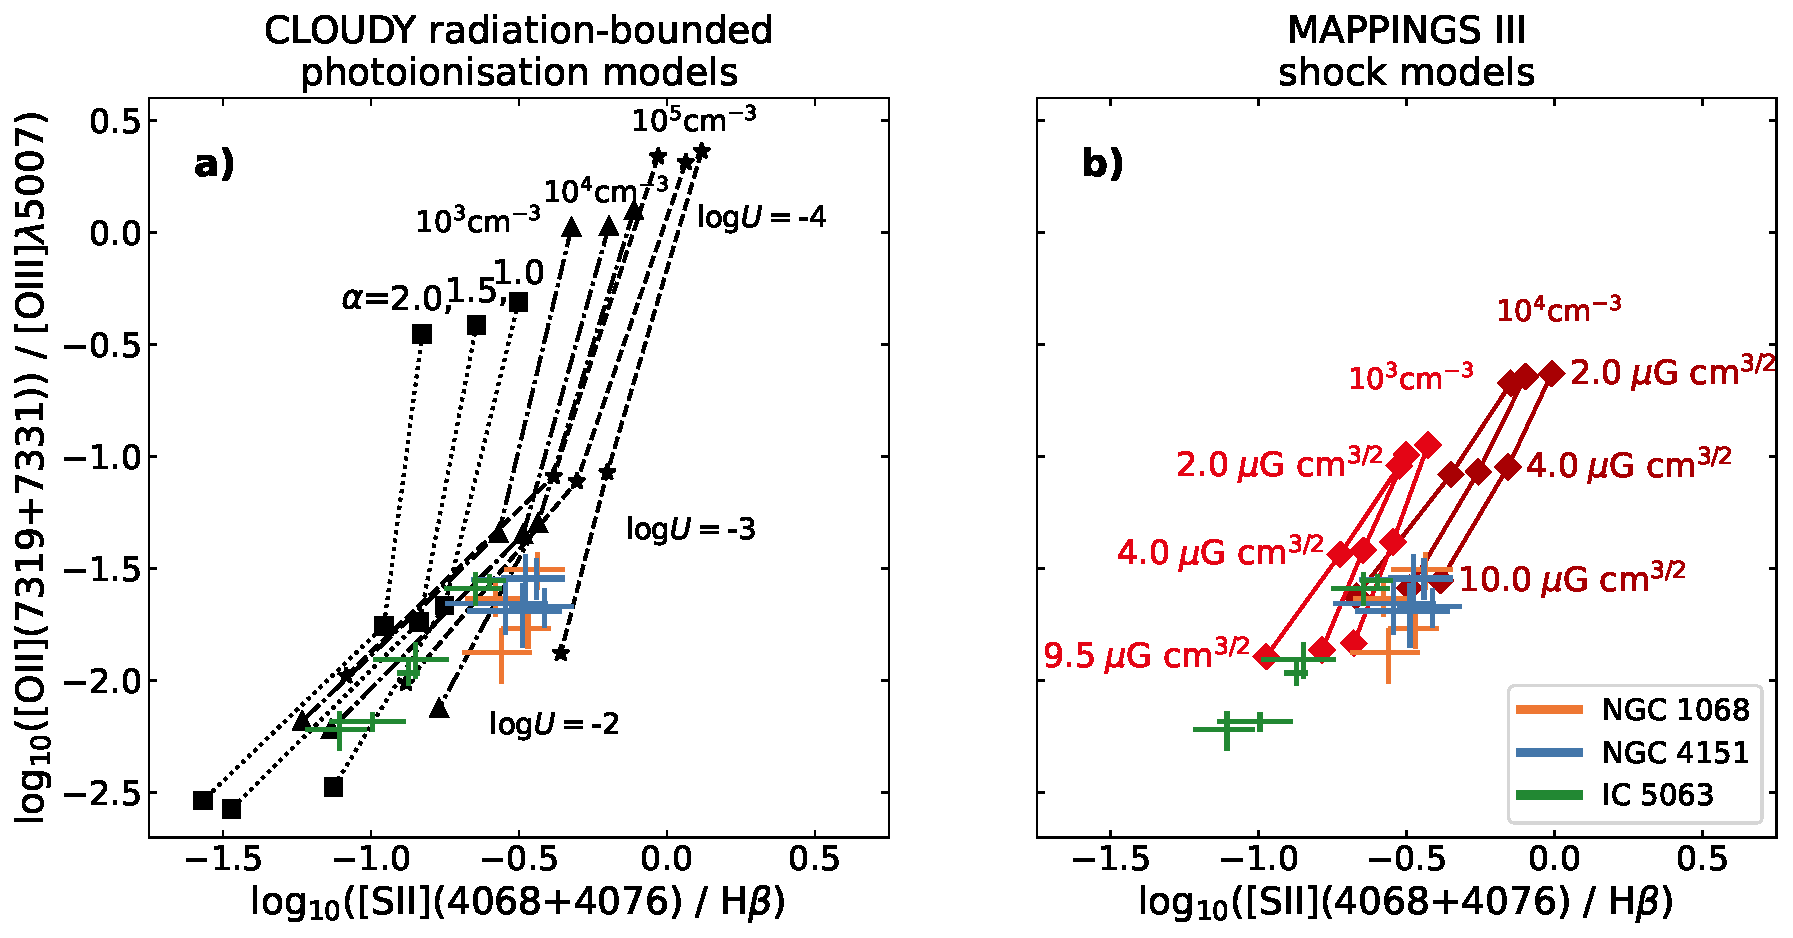
\includegraphics[width=\linewidth]{figures/stis_seyferts/tr_oiii_hbeta.pdf}
    \caption[TR({[}SII{]})/H$\mathrm{\beta}$ vs TR({[}OII{]})/{[}OIII{]}$\lambda$5007 diagnostic diagram for the warm ionised gas in IC\;5063, NGC\;1068, and NGC\;4151, along with grids produced from photo- and shock-ionisation modelling.]{TR([SII])/H$\mathrm{\beta}$ vs TR([OII])/[OIII]$\lambda$5007 ratio grids from \textsc{CLOUDY} radiation-bounded photoionisation modelling (\textbf{a}) and the \citet{Allen2008} MAPPINGS III shock-ionisation models (\textbf{b}), along with measured values for each aperture in NGC\;1068 (orange crosses), NGC\;4151 (blue crosses) and IC\;5063 (green crosses; see Chapter \ref{chapter: xshooter_ic5063}). The modelled photoionisation-line-ratio grid shown in \textbf{a)} is for three spectral indices ($\alpha=1.0, 1.5, 2.0$; labelled) at different electron densities (squares: $n_e=10^3$\;cm$^{-3}$; triangles: $n_e=10^4$\;cm$^{-3}$; stars: $n_e=10^5$\;cm$^{-3}$) and ionisation parameters (log\;$U$; labelled), while the shock-ionisation grids in \textbf{b)} are for post-shock densities of $n=10^3$\;cm$^{-3}$ and $n=10^{4}$\;cm$^{-3}$ (labelled; assuming a shock compression factor of 100), magnetic parameters of $B/\sqrt{n}=2$, 4, 10 \;$\mu$G\;cm$^{3/2}$ (labelled), and velocities of $v_\mathrm{shock}=400, 600, 800$\;km\;s$^{-1}$.}
    \label{fig: stis_seyferts: tr_oiii_hbeta}
\end{figure*}

\subsection{Comparison of the transauroral-line-derived electron densities to other techniques}
\label{section: stis_seyferts: disc-density-tr}

Using the transauroral-line method, high electron densities are measured for NGC\;1068 (4.00\;\textless\;log($n_e$[cm$^{-3}$])\;\textless\;4.75) and NGC\;4151 (3.50\;\textless\;log($n_e$[cm$^{-3}$])\;\textless\;4.10) (Section\;\ref{section: stis_seyferts: tr_diagnostics}; Table \ref{tab: stis_seyferts: ne_ebv_te}). This agrees with the similarly high densities ($n_e$\;\textgreater\;10$^3$\;cm$^{-3}$) that are derived from multi-component photoionisation modelling of both objects presented in \citet{Crenshaw2015} and \citet{Revalski2021} (see also \citealt{Collins2009} and \citealt{Revalski2022}). Crucially, the derived densities from both techniques lie above the sensitivity range of the traditional [SII](6717/6731) and [OII](3726/2739) techniques, which are commonly used (either directly or as a basis for assumption) to derive electron densities in studies of the warm ionised phase (e.g. \citealt{Nesvadba2006, Liu2013, Harrison2014, Fiore2017}), thus further supporting the need for robust warm-ionised gas electron density diagnostics such as the transauroral-line technique and multi-component photoionisation modelling.

Through the use of the traditional [SII](6717/6731) ratio, \citet{Kraemer2000II} (using the same STIS dataset as used in this work) and \citet{Kakkad2018} and \citet{Mingozzi2019} (using IFU data) derived electron densities of $n_e\sim10^3$\;cm$^{-3}$ for the outflows in the NLR of NGC\;1068. These [SII]-derived densities are 1--1.5 orders of magnitude lower than those that are found using the transauroral-line method, and are close to the upper limit of the density range for the [SII]-ratio technique (Appendix\;\ref{appendix: properties_of_warm_ionised_diagnostic_lines}: $n_{crit}\sim10^{3.5}$\;cm$^{-3}$). This provides further evidence that, for gas of electron densities $n_e$\;\textgreater\;10$^{3.5}$\;cm$^{-3}$, the [SII](6717/6731) ratio may underestimate the true electron density by more than an order of magnitude.

\subsection{The impact of the outflowing gas on the host galaxies}

Using densities derived from the transauroral-line ratios, reddening-corrected recombination line fluxes, and kinematics taken from previous modelling, mass outflow rates in the range 0.6\;\textless\;$\dot{M}_\mathrm{out}$\;\textless\;6.9\;M$_\odot$\;yr$^{-1}$ and coupling efficiencies in the range 1.1$\times10^{-3}$\;\textless\;$\epsilon_\mathrm{kin}$\;\textless\;0.99\;per\;cent are found (Table \ref{tab: energetics}). In many cases, the calculated coupling efficiencies are just above the lower limit required by models of the co-evolution of galaxies and their supermassive black holes (e.g. $\sim0.5$--10\;per\;cent: \citealt{DiMatteo2005, Springel2005, Hopkins2010}). It is important to note that there is likely more outflowing material within the bicones that is not covered by the slits (which are only 0.1\;arcseconds wide), and that comparisons between coupling efficiencies from models and observations are not straightforward (see Section\;\ref{section: introduction: outflows: comparisons_to_models} and \citealt{Harrison2018}). To properly account for the impact of the warm-ionised outflows, detailed studies that make use of robust density diagnostics, separate emission from the outflowing and quiescent gas and, importantly, cover the entire NLRs of both objects, are needed. Moreover, I highlight that assessments of \textit{all} gas phases --- not just the warm ionised phase --- are needed to robustly assess the \textit{total} impact of the AGN-driven outflows (Section\;\ref{section: introduction: outflows: energetics: multi-phase}; \citealt{Cicone2018}), as the warm-ionised gas may represent just a fraction of the total outflowing gas mass at a given radius (e.g. Chapter \ref{chapter: xshooter_ic5063}; \citealt{RamosAlmeida2019}). Therefore, it is likely that the true coupling efficiencies of the total NLR outflows in NGC\;1068 and NGC\;4151 are higher than are calculated here.

\subsection{A tale of three Seyferts: NGC 1068, NGC 4151 and IC 5063}

\begin{table*}
    \vspace*{12pt}
    \centering
    \renewcommand{\arraystretch}{1}
    \begin{tabular}{lccccc}
    \multirow{2}{*}{Object}  & \multirow{2}{*}{$L_\mathrm{bol}$ (erg\;s$^{-1}$)}    & $L_\mathrm{1.4\;GHz}$ & \multirow{2}{*}{$P_\mathrm{jet}$ (erg\;s$^{-1}$)}  & \multirow{2}{*}{$\theta_\mathrm{jet}$$^a$} & \multirow{2}{*}{Ionisation mechanism$^b$} \\ 
        &   & (W\;Hz$^{-1}$)  &   &   & \\ 
        \hline
    \multicolumn{6}{}{\vspace*{-0.2cm}}\\
    \multirow{2}{*}{NGC\;1068} & \multirow{2}{*}{0.4--4.7$\times10^{45}$} & \multirow{2}{*}{2.3$\times10^{23}$}   & \multirow{2}{*}{1.8$\times10^{43}$}   & \multirow{2}{*}{$\sim45^\circ$} & Matter-bounded  \\
        &   &   &   &   &   photoionisation \\
    \multicolumn{6}{}{\vspace*{-1cm}}\\
    \multirow{2}{*}{NGC\;4151} & \multirow{2}{*}{1.4$\times10^{44}$} & \multirow{2}{*}{1.6$\times$10$^{22}$}  & \multirow{2}{*}{$\sim10^{42}$}   & \multirow{2}{*}{$\sim36^\circ$} &  Photo- and/or \\
        &   &   &   &   &   shock-ionisation \\
    \multicolumn{6}{}{\vspace{-1cm}}\\
    \multirow{2}{*}{IC\;5063}  & \multirow{2}{*}{7.6$\times 10^{44}$}  & \multirow{2}{*}{3$\times10^{23}$} & \multirow{2}{*}{10$^{44-45}$} & \multirow{2}{*}{$\sim5^\circ$} & Radiation-bounded \\
        &   &   &   &   &   photoionisation \\
    \multicolumn{6}{}{\vspace{-1cm}}\\
    \end{tabular} \\
    $^a$Jet power for NGC\;1068: \citet{GarciaBurillo2014}; NGC\;4151: \citet{Wang2011b}; IC\;5063: \citet{Mukherjee2018}. \\
    $^b$Determined with line ratios measured in slits along $\mathrm{PA}=202^\circ$ (NGC\;1068), $\mathrm{PA}=70^\circ$ (NGC\;4151) and $\mathrm{PA}=115^\circ$ (IC\;5063). \\
    \caption{Bolometric luminosities, 1.4\;GHz radio luminosities, jet powers ($P_\mathrm{jet}$), jet orientations with respect to the disk ($\theta_\mathrm{jet}$), and ionisation mechanisms determined along the radio axes for the nearby Seyfert galaxies NGC\;1068, NGC\;4151, and IC\;5063.}
    \label{tab: three_seyferts}
\end{table*}

Finally, using the results for the nearby Seyfert 2 IC\;5063 presented in Chapter \ref{chapter: xshooter_ic5063} along with the results for NGC\;1068 and NGC\;4151 that are presented here, a sample of nearby Seyferts with spatially-resolved, detailed studies of their NLR outflows can be constructed.

IC\;5063 is a nearby ($z=0.01131$) early-type Seyfert 2 galaxy that is seen close to edge-on, with a radio jet propagating almost in the plane of the disk which drives fast (\mbox{$v_\mathrm{out}$\;\textgreater\;700\;km\,s$^{-1}$}) outflows (\citealt{Morganti1998, Oosterloo2000, Morganti2015, Mukherjee2018}; Chapter \ref{chapter: xshooter_ic5063}). These outflows are seen in multiple gas phases, including warm ionised (\citealt{Morganti2007, Sharp2010, Congiu2017, Venturi2021}; Chapter \ref{chapter: xshooter_ic5063}), neutral atomic \citep{Morganti1998, Oosterloo2000}, warm molecular (\citealt{Tadhunter2014}; Chapter \ref{chapter: xshooter_ic5063}), and cold molecular \citep{Morganti2013_IC5063, Morganti2015, Dasyra2016, Oosterloo2017}.

In Chapter \ref{chapter: xshooter_ic5063}, I presented evidence that both the outflowing and quiescent warm-ionised gas in IC\;5063 has dominant AGN-photoionisation --- even though the outflows show clear signatures of jet-acceleration --- and that the different outflow phases may represent a post-shock cooling sequence. I interpreted this situation as the pre-shock gas being AGN-photoionised, and the closest post-shock gas to the AGN being maintained in an ionised state by photoionisation. In Figure\;\ref{fig: stis_seyferts: oiii_heii_hb_seyferts}, the [OIII](5007/4363) and HeII4686/H$\mathrm{\beta}$ ratios for the outflowing gas in IC\;5063 (Section\;\ref{section: xshooter_ic5063: properties_of_outflowing_gas: uvb_vis_analysis_and_results: electron_temperatures}) are added to the diagnostic diagram presented in this chapter (Figure\;\ref{fig: stis_seyferts: oiii_heii_hbeta_stis}). Furthermore, [OII](7319+7331)/[OIII]$\lambda$5007 and [SII](4068+4076)/H$\mathrm{\beta}$ ratios for IC\;5063 (alongside NGC\;1068 and NGC\;4151) are presented in Figure\;\ref{fig: stis_seyferts: tr_oiii_hbeta}, determined using the Xshooter data for IC\;5063 --- it can be seen that they are consistent with radiation-bounded AGN-photoionisation with gas densities in the range \mbox{10$^3$\;\textless\;$n_e$\;\textless\;10$^4$\;cm$^{-3}$} and ionisation parameters in the range \mbox{$-3$\;\textless\;log\;$U$\;\textless\;$-2$}, in agreement with the values determined in Chapter \ref{chapter: xshooter_ic5063}. 

\begin{figure}[!t]
\centering
    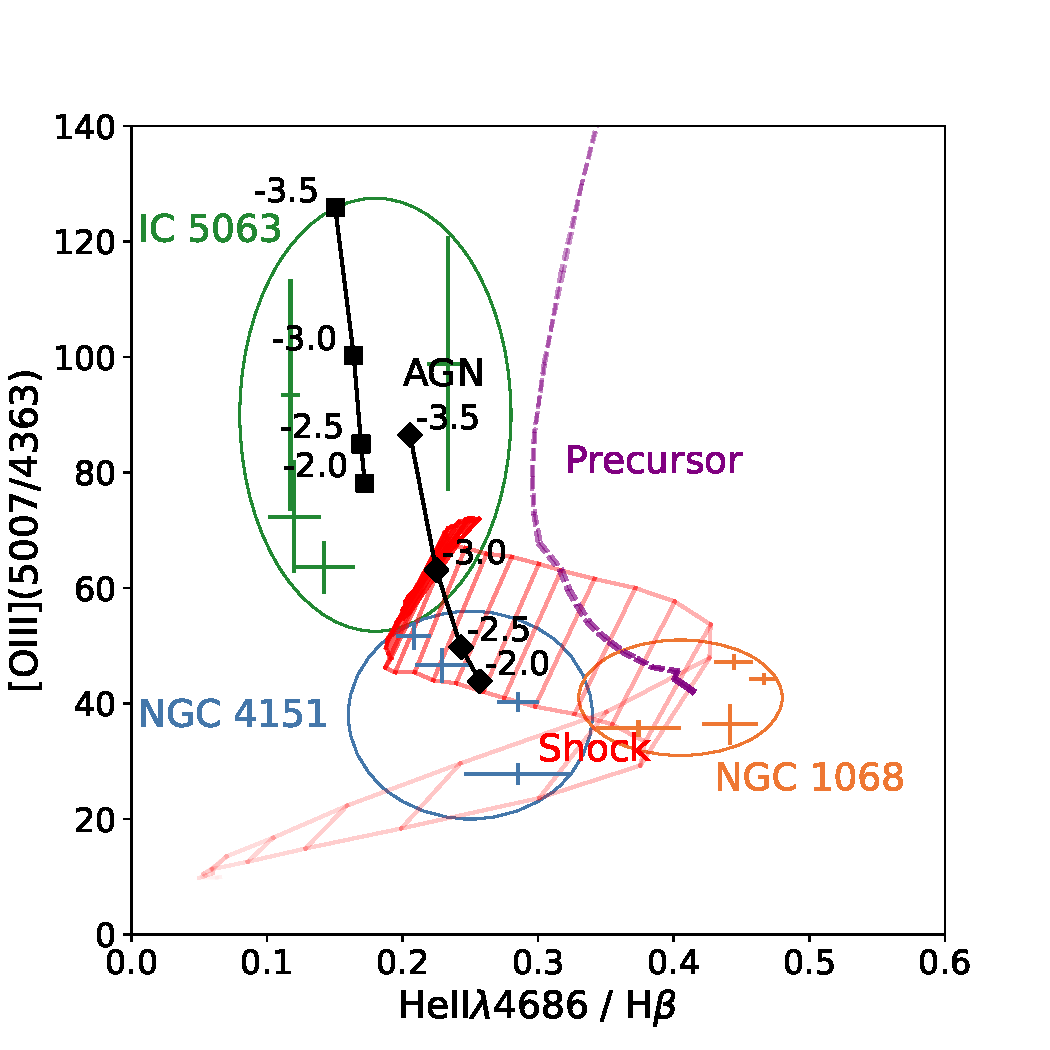
\includegraphics[width=0.8\linewidth]{figures/stis_seyferts/oiii_heii_hb_seyferts.pdf}
    \caption[HeII$\lambda$4686/H$\mathrm{\beta}$ vs {[}OIII{]}5007/{[}OIII{]}$\lambda$4363 diagnostic diagram for the warm ionised gas in IC\;5063, NGC\;1068 and NGC\;4151, including modelled values for (radiation-bounded and matter-bounded) photo- and shock-ionised gas.]{[OIII](5007/4363) vs HeII4686/H$\mathrm{\beta}$ diagnostic diagram (as in Figure\;\ref{fig: stis_seyferts: oiii_heii_hbeta_stis}) with line ratios measured from the STIS spectra of NGC\;1068 and NGC\;4151 (presented in this work), and from Xshooter spectra of IC\;5063 (Chapter \ref{chapter: xshooter_ic5063}, Figure \ref{fig: xshooter_ic5063: heii_hbeta}). The AGN, shock, and precursor models are the same as those described in Section\;\ref{section: stis_seyferts: mechanisms}. The three objects each show distinct ionisation conditions, hinting at the complex nature of the NLRs of Seyfert galaxies.}
    \label{fig: stis_seyferts: oiii_heii_hb_seyferts}
\end{figure}

It is interesting that the overall differences in ionisation conditions \textit{between} the three galaxies are significantly larger than the range of ionisation conditions \textit{within} the galaxies. This small sample thus shows three distinct cases in the three objects: radiation-bounded AGN-photoionisation in IC\;5063, matter-bounded AGN-photoionisation in NGC\;1068, and shock-ionisation or radiation-bounded AGN-photoionisation with a relatively-flat spectral index and higher ionisation parameters in NGC\;4151. Despite all being classified as Seyferts, the details of the ionisation mechanisms in the objects vary greatly. This is particularly interesting considering that in all cases, the outflows detected along the radio axes appear to be spatially confined to the radio structures (i.e. the outflows do not extend beyond the radio lobes in the NLRs). As argued in Section\;\ref{section: stis_seyferts: disc-ionisation}, this is consistent with shock-acceleration, although it does not rule out radiative-acceleration. If the outflows in IC\;5063, NGC\;1068 and NGC\;4151 are shock-accelerated, then this would highlight the importance of not deriving information regarding the outflow acceleration mechanisms based solely on the ionisation/excitation mechanisms or kinematics of the gas in NLRs: a full account, involving detailed multi-wavelength observations with multiple diagnostics, is required to properly evaluate the relative contributions of different mechanisms. 

Despite evidence that the outflows in all three objects are being driven by the radio jet, the densities of the outflowing gas differ by more than an order of magnitude: for IC\;5063, the outflowing gas has densities in the range 3.17\;\textless\;log($n_e$\;[cm$^{-3}$])\;\textless\;3.43 (Table \ref{tab: xshooter_ic5063: densities}), while for NGC\;1068 and NGC\;4151 the densities are in the ranges 4.00\;\textless\;log($n_e$\;[cm$^{-3}$])\;\textless\;4.75 and 3.50\;\textless\;log($n_e$\;[cm$^{-3}$])\;\textless\;4.10, respectively (Table \ref{tab: stis_seyferts: ne_ebv_te}). The reason for this may simply be due to different pre-shock gas densities in the different objects (assuming that the outflows in all three are shock-accelerated): for IC\;5063 the pre-shock density is 2.1\;\textless\;log($n_e$\;[cm$^{-3}$])\;\textless\;2.7, however without higher-velocity-resolution spectra, it is not possible to determine the quiescent gas densities in NGC\;1068 and NGC\;4151. In addition, the differing post-shock densities in the three Seyferts may be due to different cooling conditions behind the shock front. Standard shock-jump conditions predict a compression factor of $\sim$4, however, this may be much higher ($\sim$100) if the post-shock gas has cooled in pressure equilibrium \citep{Sutherland2017, Santoro2018}.

Moreover, it is important to note that all three objects have low-to-intermediate radio luminosities (1.6$\times10^{22}$\;\textless\;$L_\mathrm{1.4\;GHz}$\;\textless\;3.0$\times10^{23}$\;W\;Hz$^{-1}$; Table \ref{tab: three_seyferts}) --- again, if the outflows in these Seyferts are jet-accelerated, then this would reinforce the importance of jet-driven shocks as a feedback mechanism in the inner regions of galaxies, even at lower radio luminosities, in agreement with the statistical study of nearby AGN presented by \citet{Mullaney2013}. Furthermore, the radio jets in NGC\;1068 and NGC\;4151 are oriented out of the galactic disks by $\sim$45$^\circ$ and $\sim$36$^\circ$ respectively, unlike IC\;5063 in which the jet propagates almost directly into the plane of the disk. Therefore, at least within the central few-hundred parsecs of the AGN, this would show that inclined jets can still have an impact on the kinematics and ionisation of the NLR, as predicted by recent relativistic hydrodynamic simulations \citep{Mukherjee2018, Meenakshi2022b}, which show that a jet inclined $\theta_\mathrm{jet}\sim45^\circ$ to the galaxy's disk may have a significant effect on the kinematics, density, and temperature of the gas within the central few kiloparsecs (albeit less so than a jet inclined in the plane of the disk, such as is the case in IC\;5063). Similar hydrodynamic simulations, specifically tailored to the situations in NGC\;1068 and NGC\;4151, could thus be used to quantify the impact of their radio jets on the star-forming gas in their NLRs, as well as the impact of inclined kpc-scale jets in general.

Ultimately, further observations of NGC\;1068 and NGC\;4151 are required to decisively determine the outflow acceleration mechanism(s). Namely, wide-wavelength-coverage spectroscopy (to make available a range of diagnostics) with sufficient velocity resolution to kinematically-discriminate between outflowing (post-shock?) and quiescent (pre-shock?) gas.

\section{Chapter conclusions}
\label{section: stis_seyferts: conclusions}

By analysing archival HST/STIS spectra taken along the radio axes of the inner few hundred parsecs of the NLR of the prototypical Seyfert galaxies NGC\;1068 and NGC\;4151, the following was found.

\begin{itemize}
    \item Spatially-resolved electron densities in the ranges 4.00\;\textless\;log$_{10}(n_e$\;[cm$^{-3}$])\;\textless\;4.75 and 3.60\;\textless\;log$_{10}(n_e$\;[cm$^{-3}$])\;\textless\;4.10  are measured using the transauroral-line technique for the NLR gas in NGC\;1068 and NGC\;4151, respectively. These values are an order of magnitude above those commonly reported and assumed based on traditional density estimates, but are in agreement with the results from alternative diagnostics such as multi-component photoionisation modelling. Overall, these results provide further motivation for the use of the transauroral lines in deriving electron densities of AGN-driven outflows.
    \item The measured emission-line ratios for the warm-ionised gas are consistent with the dominant ionisation mechanisms being matter-bounded AGN-photoionisation in NGC\;1068, and shock-ionisation and/or radiation-bounded AGN-photoionisation with a relatively flat spectral index (and/or higher ionisation parameters and lower metallicities) in NGC\;4151.
    \item Along the radio axes, the outflows in the northeastern cones of both objects have similar spatial extents to the radio structures --- this is consistent with the outflows in their NLRs being shock-accelerated by the radio jets and reionised by radiation from the AGN, although it does not rule out radiative-acceleration.
    \item Applying the transauroral-line technique to gas that has dominant shock-ionisation may incur an uncertainty on the derived electron densities by up to $\pm0.38$ orders of magnitude, which is still far below the potential order-of-magnitude error incurred when using techniques which are not sensitive to higher-density gas. However, care must still be taken when using detailed density-diagnostic techniques, as the ionisation mechanism of the gas may alter the results. Therefore, robust ionisation-mechanism diagnostics should be used to verify the validity of the density measurements.
    \item Finally, combining these findings with those for the nearby Seyfert 2 galaxy IC\;5063 shows that ionisation mechanisms and outflow conditions along the radio axes in the central few hundred parsecs vary significantly between the different objects. Hence, overall, this chapter highlights the necessity of care when deriving information about outflow acceleration mechanisms from the ionisation of the gas, and the need for robust ionisation-mechanism diagnostics with detailed observations.
\end{itemize}

\section*{Chapter acknowledgements}
\addcontentsline{toc}{section}{\protect\numberline{}Chapter acknowledgements}

I thank the anonymous referee for their helpful comments and suggestions, which improved the clarity of the publication that this chapter is based on \citep{HoldenTadhunter2023}. Based on observations made with the NASA/ESA Hubble Space Telescope, and obtained from the Hubble Legacy Archive, which is a collaboration between the Space Telescope Science Institute (STScI/NASA), the Space Telescope European Coordinating Facility (ST-ECF/ESA) and the Canadian Astronomy Data Centre (CADC/NRC/CSA). This research has made use of the NASA/IPAC Infrared Science Archive, which is funded by the National Aeronautics and Space Administration and operated by the California Institute of Technology. This work makes use of the Starlink software \citep{Currie2014}, which is currently supported by the East Asian Observatory. For the purposes of open access, the authors have applied a Creative Commons Attribution (CC BY) licence to any Author Accepted Manuscript Arising.


\section*{Data Availability}
\addcontentsline{toc}{section}{\protect\numberline{}Data availability}

The data used in this chapter is available from the Hubble Legacy Archive (HLA) (\url{https://hla.stsci.edu/hlaview.html}) with proposal IDs GTO:5754 (PI Ford) and GTO:5124 (PI Ford) for the HST/WFPC2 [OIII] imaging, and proposal IDs GTO:7573 (PI Kraemer) and GTO:7569 (PI Hutchings) for the HST/STIS spectra.
